\documentclass{beamer}

\usefonttheme[onlymath]{serif}
\usepackage[utf8]{inputenc}
\usepackage{amsmath}
\usepackage{array}
\usepackage{graphicx}
\usepackage{mathtools}
\usepackage{minted}
\usepackage{hyperref}
\usepackage[ruled]{algorithm2e}
\hypersetup{
    colorlinks=true,
    linkcolor=blue,
}
\usemintedstyle{manni}
\newminted{python}{fontsize=\footnotesize}

\usetheme{Pittsburgh}

\usepackage{pgfpages}
\setbeamertemplate{note page}{\pagecolor{yellow!5}\insertnote}
\setbeameroption{show notes on second screen=right}

\usepackage{tikz}
\usetikzlibrary{fit}
\tikzset{%
  highlight/.style={rectangle,rounded corners,fill=red!15,draw,
    fill opacity=0.5,thick,inner sep=0pt}
}
\newcommand{\tikzmark}[2]{\tikz[overlay,remember picture,
  baseline=(#1.base)] \node (#1) {#2};}
%
\newcommand{\Highlight}[1][submatrix]{%
    \tikz[overlay,remember picture]{
    \node[highlight,fit=(left.north west) (right.south east)] (#1) {};}
}

\title{Your Neural Network for NLP is Probably Wrong}
\subtitle{Why You Need to Mask More Than You Think}
\author{Brian Lester}
\institute{Interactions}
\date{February, 27, 2020}

\def\R{\mathbb{R}}
\def\N{\mathbb{N}}
\newcommand{\softmax}{\mathop{\rm softmax}\nolimits}
\newcommand{\similar}{\mathop{\rm sim}\nolimits}
\newcommand{\logsumexp}{\mathop{\rm logsumexp}}

\begin{document}

\frame{\titlepage}
\begin{section}{Bio}

    \begin{frame}
        \frametitle{Slides}
        This QR code has a link to the slides if you want to follow along.
        \begin{center}
            
\includegraphics[height=0.8\textheight]{images/qr.png}
        \end{center}
    \end{frame}

    \begin{frame}
        \frametitle{Cats}
        \begin{center}
            
\includegraphics[height=0.8\textheight]{images/cat-qr.png}
        \end{center}
        \note{
            \begin{itemize}
                \item This QR code as a link to a compilation video of cats getting scared by cucumbers
                \item In case you want to watch this instead of paying attention to the talk
                \item Side Note: I have heard that this is very upsetting to the cats so I wouldn't recommend doing this
                    to your cat but given that these people already filmed it I don't think it is \textit{that} bad to
                    have a laugh at it.
            \end{itemize}
        }
    \end{frame}

    \begin{frame}
        \frametitle{Me}
        \begin{itemize}
            \item Work on NLP at Interactions
            \item My specialization is in Deep Learning
            \item Maintain \href{https://github.com/dpressel/mead-baseline}{Mead-Baseline}
        \end{itemize}
        \note{
            \begin{itemize}
                \item This is my ``Why you should listen to me'' slide
                \item I do NLP at interactions where we use NLP to ``facilitate customer care interactions'' aka build better chat bots
                \item My specialization is DL and We use DL for most models so I have a lot of experience
                \item I help maintain Mead-Baseline, our open-source Deep Learning modeling software so I have a lot of
                    experience writing Neural Networks for NLP
                \item I have batched some complex operations for Mead-Baseline
                \begin{itemize}
                    \item Batched the CRF
                    \item Batched Beam Search
                \end{itemize}
                \item I have tracked down a lot of hidden batch instability problems
                \item I am trying to get more involved with research so if anyone needs help with some idea, especially if
                    the implementation is tricky, hit me up.
            \end{itemize}
        }
    \end{frame}

\end{section} % Bio

\begin{section}{Motivation}
    \begin{subsection}{What is batching?}
        \begin{frame}
            \frametitle{Binary Logistic Regression}
            \begin{align*}
                n &\coloneqq \text{number of features} \\
                c &\coloneqq \text{number of class} \coloneqq 1 \\
                f &\in \R ^ {n} \\
                w &\in \R ^ {n} \\
                s &= \sum_{i=0}^{n} f_i * w_i \\
            \end{align*}
        \note{
            \begin{itemize}
                \item First I'm going to build up batching through building examples by starting with Binary LR
                \item In binary LR we have a vector representing features and a vector of the same size representing
                    weights
                \item (Normally in NLP we have sparse features where we don't have a actual vector of features, we would use
                    something like a hashmap instead, but inside a neural network everything is dense vectors so we will use
                    dense vectors here because it is just a pedagogical example)
                \item We take the sum of the features weighted by the weight to create a score which we call a logit.
                \item This operation is called the dot product.
                \item Normally we then us a function like sigmoid to create a final probability (and then calculate
                    losses and gradients) but we don't need to worry about that for this example.
            \end{itemize}
        }
        \end{frame}

\begin{frame}[fragile]
    \frametitle{Binary Logistic Regression}
    \begin{pythoncode}
                        s = np.dot(f, w)
    \end{pythoncode}
    \note{
        \begin{itemize}
            \item In this example we are representing our feature and weights as numpy vectors
            \item W can use the dot product function which to calculate the sum of the element wise products of the
                vectors.
        \end{itemize}
    }
\end{frame}

        \begin{frame}
            \frametitle{Binary Logistic Regression}
            \begin{align*}
                f &= \left[ \begin{array}{*6{c}}
                    & 1 & 2 & 3 & 4 &
                    \end{array}
                    \right] \\
                w &= \left[ \begin{array}{*6{c}}
                    & 5 & 6 & 7 & 8 &
                    \end{array}
                    \right] \\
                s &=
            \end{align*}
            \note{
                \begin{itemize}
                    \item Here we can see our feature vector and our weight vector
                    \item Now lets look at the mechanics of what is happening in our dot product calculation
                \end{itemize}
            }
        \end{frame}

        \begin{frame}
            \frametitle{Binary Logistic Regression}
            \begin{align*}
                f &= \left[ \begin{array}{*6{c}}
                    &\tikzmark{left}{1}\tikzmark{right} & 2 & 3 & 4 &
                    \end{array}
                    \right] \\
                \Highlight[first]
                w &= \left[ \begin{array}{*6{c}}
                    &\tikzmark{left}{5}\tikzmark{right} & 6 & 7 & 8 &
                    \end{array}
                    \right] \\
                \Highlight[second]
                s &= 5
            \end{align*}
            \note{
                \begin{itemize}
                    \item We multiply these terms together and add the result into the s
                \end{itemize}
            }
        \end{frame}

        \begin{frame}
            \frametitle{Binary Logistic Regression}
            \begin{align*}
                f &= \left[ \begin{array}{*6{c}}
                    & 1 & \tikzmark{left}{2} \tikzmark{right}{} & 3 & 4 &
                    \end{array}
                    \right] \\
                \Highlight[first]
                w &= \left[ \begin{array}{*6{c}}
                    & 5 & \tikzmark{left}{6} \tikzmark{right}{} & 7 & 8 &
                    \end{array}
                    \right] \\
                \Highlight[second]
                s &= 17
            \end{align*}
            \note{
                \begin{itemize}
                    \item And it continues on like this.
                \end{itemize}
            }
        \end{frame}

        \begin{frame}
            \frametitle{Binary Logistic Regression}
            \begin{align*}
                f &= \left[ \begin{array}{*6{c}}
                    & \tikzmark{left}{1} & 2 & 3 & \tikzmark{right}{4} &
                    \end{array}
                    \right] \\
                \Highlight[first]
                w &= \left[ \begin{array}{*6{c}}
                    & \tikzmark{left}{5} & 6 & 7 & \tikzmark{right}{8} &
                    \end{array}
                    \right] \\
                \Highlight[second]
                s &= 70
            \end{align*}
            \note{
                \begin{itemize}
                    \item Here we highlight the elements in these arrays that interact with each other in our dot
                        product.
                \end{itemize}
            }
        \end{frame}

        \begin{frame}
            \frametitle{Multi-class Logistic Regression}
            \begin{align*}
                n &\coloneqq \text{number of features} \\
                c &\coloneqq \text{number of class} \\
                f &\in \R ^ {n} \\
                W &\in \R ^ {n \text{ x } c} \\
                s &\in \R ^ {c} \\
                \forall_{j \in c}\hspace{2pt} s_j &= \sum_{i=0}^{n} f_i * W_{ij} \\
            \end{align*}
            \note{
                \begin{itemize}
                    \item We now extend to multi-class LR
                    \begin{itemize}
                        \item In binary LR we are deciding between to things for example Positive or Negative sentiment
                        \item In multi-class LR we are deciding between multi classes, for example Science, Technology,
                            Politics, cooking, and video games for document classification
                    \end{itemize}
                    \item We still have a feature vector for some document.
                    \item We now have multiple weight vectors, one for each class
                    \item We pack our weight vectors into a single matrix of size n (the number of features we have) by c (which is the number of classes
                        we have).
                    \item Now our logits are a vector, we have a score for each class
                    \item for each class we do this dot product between the feature vector and one of the weight
                        vectors
                    \item Once we have the score we normally turn it into probabilities with the softmax function but we
                        can skip this for this example.
                \end{itemize}
            }

        \end{frame}

\begin{frame}[fragile]
    \frametitle{Multi-class Logistic Regression}
    \begin{pythoncode}
                    s = []
                    for w in W.T:
                        s.append(np.dot(f, w))
                    s = np.array(s)
    \end{pythoncode}
    \note{
        \begin{itemize}
            \item Here we see code that calculates the logits how I described it before.
            \item where we explicitly do the dot between the feature and each weight vector in turn
            \item We turn the results into a vector at the end
        \end{itemize}
    }
\end{frame}

\begin{frame}[fragile]
    \frametitle{Multi-class Logistic Regression}
    \begin{pythoncode}
                    s = np.dot(f, W)
    \end{pythoncode}
    \note{
        \begin{itemize}
            \item But it turns out we can actually do this in a single dot product! Lets see why
        \end{itemize}
    }
\end{frame}

        \begin{frame}
            \frametitle{Multi-class Logistic Regression}
            \begin{align*}
                f &= \left[ \begin{array}{*6{c}}
                    & 1 & 2 & 3 & 4 &
                    \end{array}
                    \right] \\
                W &= \left[ \begin{array}{*4{c}}
                    & 5 & 9  & \\
                    & 6 & 10 & \\
                    & 7 & 11 & \\
                    & 8 & 12 &
                    \end{array}
                    \right] \\
                s &= \left[ \begin{array}{*4{c}}
                    & & &
                    \end{array}
                    \right] \\
            \end{align*}
            \note{
                \begin{itemize}
                    \item Here we can see our feature vector again and see our new weight matrix
                    \item Note how the weight matrix is two weight vectors next to each other
                    \item The first column is the same weight vector we saw earlier
                    \item Lets explore how the elements of the feature vector and weight matrix are combined
                \end{itemize}
            }
        \end{frame}

        \begin{frame}
            \frametitle{Multi-class Logistic Regression}
            \begin{align*}
                f &= \left[ \begin{array}{*6{c}}
                    & \tikzmark{left}{1}\tikzmark{right}{} & 2 & 3 & 4 &
                    \end{array}
                    \right] \\
                \Highlight[first]
                W &= \left[ \begin{array}{*4{c}}
                    & \tikzmark{left}{5}\tikzmark{right}{} & 9  & \\
                    & 6 & 10 & \\
                    & 7 & 11 & \\
                    & 8 & 12 &
                    \end{array}
                    \right] \\
                \Highlight[second]
                s &= \left[ \begin{array}{*4{c}}
                    & \tikzmark{left}{5} \tikzmark{right}{} & &
                    \end{array}
                    \right] \\
                \Highlight[third]
            \end{align*}
            \note{
                \begin{itemize}
                    \item Here we can see that we multiply an element from the feature vector and the first column of
                        the weight matrix
                    \item We save this value into the score vector
                \end{itemize}
            }
        \end{frame}

        \begin{frame}
            \frametitle{Multi-class Logistic Regression}
            \begin{align*}
                f &= \left[ \begin{array}{*6{c}}
                    & 1 & \tikzmark{left}{2} \tikzmark{right}{} & 3 & 4 &
                    \end{array}
                    \right] \\
                \Highlight[first]
                W &= \left[ \begin{array}{*4{c}}
                    & 5 & 9  & \\
                    & \tikzmark{left}{6}\tikzmark{right}{} & 10 & \\
                    & 7 & 11 & \\
                    & 8 & 12 &
                    \end{array}
                    \right] \\
                \Highlight[second]
                s &= \left[ \begin{array}{*4{c}}
                    & \tikzmark{left}{17} \tikzmark{right}{} & &
                    \end{array}
                    \right] \\
                \Highlight[thrid]
            \end{align*}
            \note{
                \begin{itemize}
                    \item And it goes on like this...
                \end{itemize}
            }
        \end{frame}


        \begin{frame}
            \frametitle{Multi-class Logistic Regression}
            \begin{align*}
                f &= \left[ \begin{array}{*6{c}}
                    & \tikzmark{left}{1} & 2 & 3 & \tikzmark{right}{4} &
                    \end{array}
                    \right] \\
                \Highlight[first]
                W &= \left[ \begin{array}{*4{c}}
                    & \tikzmark{left}{5} & 9  & \\
                    & 6 & 10 & \\
                    & 7 & 11 & \\
                    & \tikzmark{right}{8} & 12 &
                    \end{array}
                    \right] \\
                \Highlight[second]
                s &= \left[ \begin{array}{*4{c}}
                    & \tikzmark{left}{70}\tikzmark{right}{} & &
                    \end{array}
                    \right] \\
                \Highlight[third]
            \end{align*}
            \note{
                \begin{itemize}
                    \item We see here that the value in this first spot of the logits was calculated between the feature
                        vector and the first column in the weight matrix
                \end{itemize}
            }
        \end{frame}

        \begin{frame}
            \frametitle{Multi-class Logistic Regression}
            \begin{align*}
                f &= \left[ \begin{array}{*6{c}}
                    & \tikzmark{left}{1}\tikzmark{right}{} & 2 & 3 & 4 &
                    \end{array}
                    \right] \\
                    \Highlight[first]
                W &= \left[ \begin{array}{*4{c}}
                    & 5 & \tikzmark{left}{9}\tikzmark{right}{}  & \\
                    & 6 & 10 & \\
                    & 7 & 11 & \\
                    & 8 & 12 &
                    \end{array}
                    \right] \\
                    \Highlight[second]
                s &= \left[ \begin{array}{*4{c}}
                    & 70 & \tikzmark{left}{9}\tikzmark{right}{} &
                    \end{array}
                    \right] \\
                    \Highlight[third]
            \end{align*}
            \note{
                \begin{itemize}
                    \item Here we see the elements of the feature vector and the second column weight matrix are
                        combined and saved into the second element of the logit vector
                \end{itemize}
            }
        \end{frame}

        \begin{frame}
            \frametitle{Multi-class Logistic Regression}
            \begin{align*}
                f &= \left[ \begin{array}{*6{c}}
                    & 1 & \tikzmark{left}{2}\tikzmark{right}{} & 3 & 4 &
                    \end{array}
                    \right] \\
                \Highlight[first]
                W &= \left[ \begin{array}{*4{c}}
                    & 5 & 9 & \\
                    & 6 & \tikzmark{left}{10}\tikzmark{right}{}  & \\
                    & 7 & 11 & \\
                    & 8 & 12 &
                    \end{array}
                    \right] \\
                \Highlight[second]
                s &= \left[ \begin{array}{*4{c}}
                    & 70 & \tikzmark{left}{29}\tikzmark{right}{} &
                    \end{array}
                    \right] \\
                \Highlight[thrid]
            \end{align*}
            \note{
                \begin{itemize}
                    \item And it goes on like this...
                \end{itemize}
            }
        \end{frame}

        \begin{frame}
            \frametitle{Multi-class Logistic Regression}
            \begin{align*}
                f &= \left[ \begin{array}{*6{c}}
                    & \tikzmark{left}{1} & 2 & 3 & \tikzmark{right}{4} &
                    \end{array}
                    \right] \\
                \Highlight[first]
                W &= \left[ \begin{array}{*4{c}}
                    & 5 & \tikzmark{left}{9}  & \\
                    & 6 & 10 & \\
                    & 7 & 11 & \\
                    & 8 & \tikzmark{right}{12} &
                    \end{array}
                    \right] \\
                \Highlight[second]
                s &= \left[ \begin{array}{*4{c}}
                    & 70 & \tikzmark{left}{110}\tikzmark{right}{} &
                    \end{array}
                    \right] \\
                \Highlight[third]
            \end{align*}
            \note{
                \begin{itemize}
                    \item We see here that the value in the second spot of the logits was calculated between the feature
                        vector and the second column in the weight matrix
                    \item So we can see here that we can calculate the logits for multiple classes at once between there
                        is no interaction between the columns of the matrix in vector-matrix multiplication.
                \end{itemize}
            }
        \end{frame}

        \begin{frame}
            \frametitle{Batched Multi-class Logistic Regression}
            \begin{align*}
                n &\coloneqq \text{number of features} \\
                c &\coloneqq \text{number of class} \\
                b &\coloneqq \text{number of examples} \\
                F &\in \R ^ {b \text{ x } n} \\
                W &\in \R ^ {n \text{ x } c} \\
                S &\in \R ^ {b \text{ x } c} \\
                \forall_{k \in b} \hspace{2pt} \forall_{j \in c} \hspace{2pt} S_{kj} &= \sum_{i=0}^{n} F_{ki} * W_{ij} \\
            \end{align*}
            \note{
                \begin{itemize}
                    \item We just saw how you can calculate the scores for multiple classes for a single example in a
                        single vector-matrix multiply. Now we will see how you can actually do this for multiple
                        examples at once.
                    \item Here we see Batched Multi-class Logistic Regression.
                    \item This means that we are doing multi-class LR but will process multiple examples at once
                    \item Like before we still have a weight matrix of $n$ by $c$
                    \item In this case we have $b$ examples
                    \item Now we have stacked multiple feature vectors into a feature matrix with $b$ rows where each row
                        represents a different feature vector.
                    \item Now our scores are a matrix were each row is the scores for an example and each column is the
                        score for some class
                    \item We could calculate this by doing the dot product of each feature vector and the weight matrix
                        and stacking the results into our score matrix
                \end{itemize}
            }
        \end{frame}

\begin{frame}[fragile]
    \frametitle{Batched Multi-class Logistic Regression}
    \begin{pythoncode}
                S = []
                for f in F:
                    S.append(np.dot(f, W))
                S = np.stack(S)
    \end{pythoncode}
    \note{
        \begin{itemize}
            \item Here we see a straight forward way to do this, where we loop over the features and calculate the
                scores for each example separately.
            \item The dot product of the feature vector and weight matrix returns a vector
            \item We collect these vectors and stack them into a single array
        \end{itemize}
    }
\end{frame}

\begin{frame}[fragile]
    \frametitle{Batched Multi-class Logistic Regression}
    \begin{pythoncode}
                S = np.dot(F, W)
    \end{pythoncode}
    \note{
        \begin{itemize}
            \item But we can actually do one better, we can calculate the whole thing, all classes for all examples in a
                single shot!
            \item Lets take a closer look
        \end{itemize}
    }
\end{frame}

        \begin{frame}
            \frametitle{Batched Multi-class Logistic Regression}
            \begin{align*}
                F &= \left[ \begin{array}{*6{c}}
                    & 1 & 2 & 3 & 4 & \\
                    & 13 & 14 & 15 & 16 &
                    \end{array}
                    \right] \\
                W &= \left[ \begin{array}{*4{c}}
                    & 5 & 9  & \\
                    & 6 & 10 & \\
                    & 7 & 11 & \\
                    & 8 & 12 &
                    \end{array}
                    \right] \\
                s &= \left[ \begin{array}{*4{c}}
                    & & & \\
                    & & &
                    \end{array}
                    \right] \\
            \end{align*}
            \note{
                \begin{itemize}
                    \item Here we see our new feature matrix is two feature vectors stacked on top of each other
                    \item Our weight matrix is still a n by c matrix of weight vectors standing next to each other
                    \item We are now doing matrix matrix multiplication
                \end{itemize}
            }
        \end{frame}

        \begin{frame}
            \frametitle{Batched Multi-class Logistic Regression}
            \begin{align*}
                F &= \left[ \begin{array}{*6{c}}
                    & \tikzmark{left}{1}\tikzmark{right}{} & 2 & 3 & 4 & \\
                    & 13 & 14 & 15 & 16 &
                    \end{array}
                    \right] \\
                \Highlight[first]
                W &= \left[ \begin{array}{*4{c}}
                    & \tikzmark{left}{5}\tikzmark{right}{} & 9  & \\
                    & 6 & 10 & \\
                    & 7 & 11 & \\
                    & 8 & 12 &
                    \end{array}
                    \right] \\
                \Highlight[second]
                s &= \left[ \begin{array}{*4{c}}
                    & \tikzmark{left}{5} \tikzmark{right}{} & & \\
                    & & &
                    \end{array}
                    \right] \\
                \Highlight[third]
            \end{align*}
            \note{
                \begin{itemize}
                    \item Here we see the values for the first class of the first example are computed using the values in the first
                        row of the feature vector and the first column of the weight matrix
                \end{itemize}
            }
        \end{frame}

        \begin{frame}
            \frametitle{Batched Multi-class Logistic Regression}
            \begin{align*}
                F &= \left[ \begin{array}{*6{c}}
                    & 1 & \tikzmark{left}{2}\tikzmark{right}{} & 3 & 4 & \\
                    & 13 & 14 & 15 & 16 &
                    \end{array}
                    \right] \\
                \Highlight[first]
                W &= \left[ \begin{array}{*4{c}}
                    & 5 & 9 \\
                    & \tikzmark{left}{6}\tikzmark{right}{} & 10  & \\
                    & 7 & 11 & \\
                    & 8 & 12 &
                    \end{array}
                    \right] \\
                \Highlight[second]
                s &= \left[ \begin{array}{*4{c}}
                    & \tikzmark{left}{17} \tikzmark{right}{} & & \\
                    & & &
                    \end{array}
                    \right] \\
                \Highlight[third]
            \end{align*}
            \note{
                \begin{itemize}
                    \item Here we see the values for the first class of the first example are computed using the values in the first
                        row of the feature vector and the first column of the weight matrix
                \end{itemize}
            }
        \end{frame}

        \begin{frame}
            \frametitle{Batched Multi-class Logistic Regression}
            \begin{align*}
                F &= \left[ \begin{array}{*6{c}}
                    & \tikzmark{left}{1} & 2 & 3 & \tikzmark{right}{4} & \\
                    & 13 & 14 & 15 & 16 &
                    \end{array}
                    \right] \\
                \Highlight[first]
                W &= \left[ \begin{array}{*4{c}}
                    & \tikzmark{left}{5} & 9  & \\
                    & 6 & 10 & \\
                    & 7 & 11 & \\
                    & \tikzmark{right}{8} & 12 &\\
                    \end{array}
                    \right] \\
                \Highlight[second]
                s &= \left[ \begin{array}{*4{c}}
                    & \tikzmark{left}{70} \tikzmark{right}{} & & \\
                    & & &
                    \end{array}
                    \right] \\
                \Highlight[third]
            \end{align*}
            \note{
                \begin{itemize}
                    \item Here we see the values for the first class of the first example are computed using the values in the first
                        row of the feature vector and the first column of the weight matrix
                \end{itemize}
            }
        \end{frame}

        \begin{frame}
            \frametitle{Batched Multi-class Logistic Regression}
            \begin{align*}
                F &= \left[ \begin{array}{*6{c}}
                    & \tikzmark{left}{1}\tikzmark{right}{} & 2 & 3 & 4 & \\
                    & 13 & 14 & 15 & 16 &
                    \end{array}
                    \right] \\
                \Highlight[first]
                W &= \left[ \begin{array}{*4{c}}
                    & 5 & \tikzmark{left}{9}\tikzmark{right}{} & \\
                    & 6 & 10 & \\
                    & 7 & 11 & \\
                    & 8 & 12 &
                    \end{array}
                    \right] \\
                \Highlight[second]
                s &= \left[ \begin{array}{*4{c}}
                    & 70 & \tikzmark{left}{9} \tikzmark{right}{} & \\
                    & & &
                    \end{array}
                    \right] \\
                \Highlight[third]
            \end{align*}
            \note{
                \begin{itemize}
                    \item Here we see the values for the second class of the first example are computed using the values in the first
                        row of the feature vector and the second column of the weight matrix
                \end{itemize}
            }
        \end{frame}

        \begin{frame}
            \frametitle{Batched Multi-class Logistic Regression}
            \begin{align*}
                F &= \left[ \begin{array}{*6{c}}
                    & 1 & \tikzmark{left}{2}\tikzmark{right}{} & 3 & 4 & \\
                    & 13 & 14 & 15 & 16 &
                    \end{array}
                    \right] \\
                \Highlight[first]
                W &= \left[ \begin{array}{*4{c}}
                    & 5 & 9 \\
                    & 6 & \tikzmark{left}{10}\tikzmark{right}{} & \\
                    & 7 & 11 & \\
                    & 8 & 12 &
                    \end{array}
                    \right] \\
                \Highlight[second]
                s &= \left[ \begin{array}{*4{c}}
                    & 70 & \tikzmark{left}{29} \tikzmark{right}{} & \\
                    & & &
                    \end{array}
                    \right] \\
                \Highlight[third]
            \end{align*}
            \note{
                \begin{itemize}
                    \item Here we see the values for the second class of the first example are computed using the values in the first
                        row of the feature vector and the second column of the weight matrix
                \end{itemize}
            }
        \end{frame}

        \begin{frame}
            \frametitle{Batched Multi-class Logistic Regression}
            \begin{align*}
                F &= \left[ \begin{array}{*6{c}}
                    & \tikzmark{left}{1} & 2 & 3 & \tikzmark{right}{4} & \\
                    & 13 & 14 & 15 & 16 &
                    \end{array}
                    \right] \\
                \Highlight[first]
                W &= \left[ \begin{array}{*4{c}}
                    & 5 & \tikzmark{left}{9} & \\
                    & 6 & 10 & \\
                    & 7 & 11 & \\
                    & 8 & \tikzmark{right}{12} &
                    \end{array}
                    \right] \\
                \Highlight[second]
                s &= \left[ \begin{array}{*4{c}}
                    & 70 & \tikzmark{left}{110} \tikzmark{right}{} & \\
                    & & &
                    \end{array}
                    \right] \\
                \Highlight[third]
            \end{align*}
            \note{
                \begin{itemize}
                    \item Here we see the values for the second class of the first example are computed using the values in the first
                        row of the feature vector and the second column of the weight matrix
                \end{itemize}
            }
        \end{frame}

        \begin{frame}
            \frametitle{Batched Multi-class Logistic Regression}
            \begin{align*}
                F &= \left[ \begin{array}{*6{c}}
                    & 1 & 2 & 3 & 4 & \\
                    & \tikzmark{left}{13}\tikzmark{right}{} & 14 & 15 & 16 &
                    \end{array}
                    \right] \\
                \Highlight[first]
                W &= \left[ \begin{array}{*4{c}}
                    & \tikzmark{left}{5}\tikzmark{right}{} & 9  & \\
                    & 6 & 10 & \\
                    & 7 & 11 & \\
                    & 8 & 12 &
                    \end{array}
                    \right] \\
                \Highlight[second]
                s &= \left[ \begin{array}{*4{c}}
                    & 70 & 110 & \\
                    & \tikzmark{left}{65}\tikzmark{right}{} & &
                    \end{array}
                    \right] \\
                \Highlight[third]
            \end{align*}
            \note{
                \begin{itemize}
                    \item Here we see the values for the first class of the second example are computed using the values
                        in the second row of the feature vector and the first column of the weight matrix
                \end{itemize}
            }
        \end{frame}

        \begin{frame}
            \frametitle{Batched Multi-class Logistic Regression}
            \begin{align*}
                F &= \left[ \begin{array}{*6{c}}
                    & 1 & 2 & 3 & 4 & \\
                    & 13 & \tikzmark{left}{14}\tikzmark{right}{} & 15 & 16 &
                    \end{array}
                    \right] \\
                \Highlight[first]
                W &= \left[ \begin{array}{*4{c}}
                    & 5 & 9 \\
                    & \tikzmark{left}{6}\tikzmark{right}{} & 10 & \\
                    & 7 & 11 & \\
                    & 8 & 12 &
                    \end{array}
                    \right] \\
                \Highlight[second]
                s &= \left[ \begin{array}{*4{c}}
                    & 70 & 110 & \\
                    & \tikzmark{left}{149}\tikzmark{right}{} & &
                    \end{array}
                    \right] \\
                \Highlight[third]
            \end{align*}
            \note{
                \begin{itemize}
                    \item Here we see the values for the first class of the second example are computed using the values
                        in the second row of the feature vector and the first column of the weight matrix
                \end{itemize}
            }
        \end{frame}

        \begin{frame}
            \frametitle{Batched Multi-class Logistic Regression}
            \begin{align*}
                F &= \left[ \begin{array}{*6{c}}
                    & 1 & 2 & 3 & 4 & \\
                    & \tikzmark{left}{13} & 14 & 15 & \tikzmark{right}{16} &
                    \end{array}
                    \right] \\
                \Highlight[first]
                W &= \left[ \begin{array}{*4{c}}
                    & \tikzmark{left}{5} & 9  & \\
                    & 6 & 10 & \\
                    & 7 & 11 & \\
                    & \tikzmark{right}{8} & 12 &
                    \end{array}
                    \right] \\
                \Highlight[second]
                s &= \left[ \begin{array}{*4{c}}
                    & 70 & 110 & \\
                    & \tikzmark{left}{382}\tikzmark{right}{} & &
                    \end{array}
                    \right] \\
                \Highlight[third]
            \end{align*}
            \note{
                \begin{itemize}
                    \item Here we see the values for the first class of the second example are computed using the values
                        in the second row of the feature vector and the first column of the weight matrix
                \end{itemize}
            }
        \end{frame}

        \begin{frame}
            \frametitle{Batched Multi-class Logistic Regression}
            \begin{align*}
                F &= \left[ \begin{array}{*6{c}}
                    & 1 & 2 & 3 & 4 & \\
                    & \tikzmark{left}{13}\tikzmark{right}{} & 14 & 15 & 16 &
                    \end{array}
                    \right] \\
                \Highlight[first]
                W &= \left[ \begin{array}{*4{c}}
                    & 5 & \tikzmark{left}{9}\tikzmark{right}{} & \\
                    & 6 & 10 & \\
                    & 7 & 11 & \\
                    & 8 & 12 &
                    \end{array}
                    \right] \\
                \Highlight[second]
                s &= \left[ \begin{array}{*4{c}}
                    & 70 & 110 & \\
                    & 382 & \tikzmark{left}{117} \tikzmark{right}{}&
                    \end{array}
                    \right] \\
                \Highlight[third]
            \end{align*}
            \note{
                \begin{itemize}
                    \item Here we see the values for the second class of the second example are computed using the values
                        in the second row of the feature vector and the second column of the weight matrix
                \end{itemize}
            }
        \end{frame}

        \begin{frame}
            \frametitle{Batched Multi-class Logistic Regression}
            \begin{align*}
                F &= \left[ \begin{array}{*6{c}}
                    & 1 & 2 & 3 & 4 & \\
                    & 13 & \tikzmark{left}{14}\tikzmark{right}{} & 15 & 16 &
                    \end{array}
                    \right] \\
                \Highlight[first]
                W &= \left[ \begin{array}{*4{c}}
                    & 5 & 9 \\
                    & 6 & \tikzmark{left}{10}\tikzmark{right}{} & \\
                    & 7 & 11 & \\
                    & 8 & 12 &
                    \end{array}
                    \right] \\
                \Highlight[second]
                s &= \left[ \begin{array}{*4{c}}
                    & 70 & 110 & \\
                    & 382 & \tikzmark{left}{117} \tikzmark{right}{}&
                    \end{array}
                    \right] \\
                \Highlight[third]
            \end{align*}
            \note{
                \begin{itemize}
                    \item Here we see the values for the second class of the second example are computed using the values
                        in the second row of the feature vector and the second column of the weight matrix
                \end{itemize}
            }
        \end{frame}

        \begin{frame}
            \frametitle{Batched Multi-class Logistic Regression}
            \begin{align*}
                F &= \left[ \begin{array}{*6{c}}
                    & 1 & 2 & 3 & 4 & \\
                    & \tikzmark{left}{13} & 14 & 15 & \tikzmark{right}{16} &
                    \end{array}
                    \right] \\
                \Highlight[first]
                W &= \left[ \begin{array}{*4{c}}
                    & 5 & \tikzmark{left}{9} & \\
                    & 6 & 10 & \\
                    & 7 & 11 & \\
                    & 8 & \tikzmark{right}{12} &
                    \end{array}
                    \right] \\
                \Highlight[second]
                s &= \left[ \begin{array}{*4{c}}
                    & 70 & 110 & \\
                    & 382 & \tikzmark{left}{614} \tikzmark{right}{}&
                    \end{array}
                    \right] \\
                \Highlight[third]
            \end{align*}
            \note{
                \begin{itemize}
                    \item And finally the last elements uses the two unused rows and columns.
                    \item So here we have seen that we can stack independent examples together just like we could stack
                        together independent weight vectors to calculate the scores for multiple examples at once.
                    \item This works because the rows and columns in matrix-matrix multiplication all act independently
                        of each other.
                    \item This means we can put otally unrelated data an be next to each other and they won't interact as it flows through
                        your network
                    \item Running multiple examples like this is what we mean by batching.
                \end{itemize}
            }
        \end{frame}


    \end{subsection} % What

    \begin{subsection}{Why Batching?}

        \begin{frame}
            \frametitle{Full Gradient Descent}

            \begin{columns}
                \begin{column}{0.5\textwidth}
                    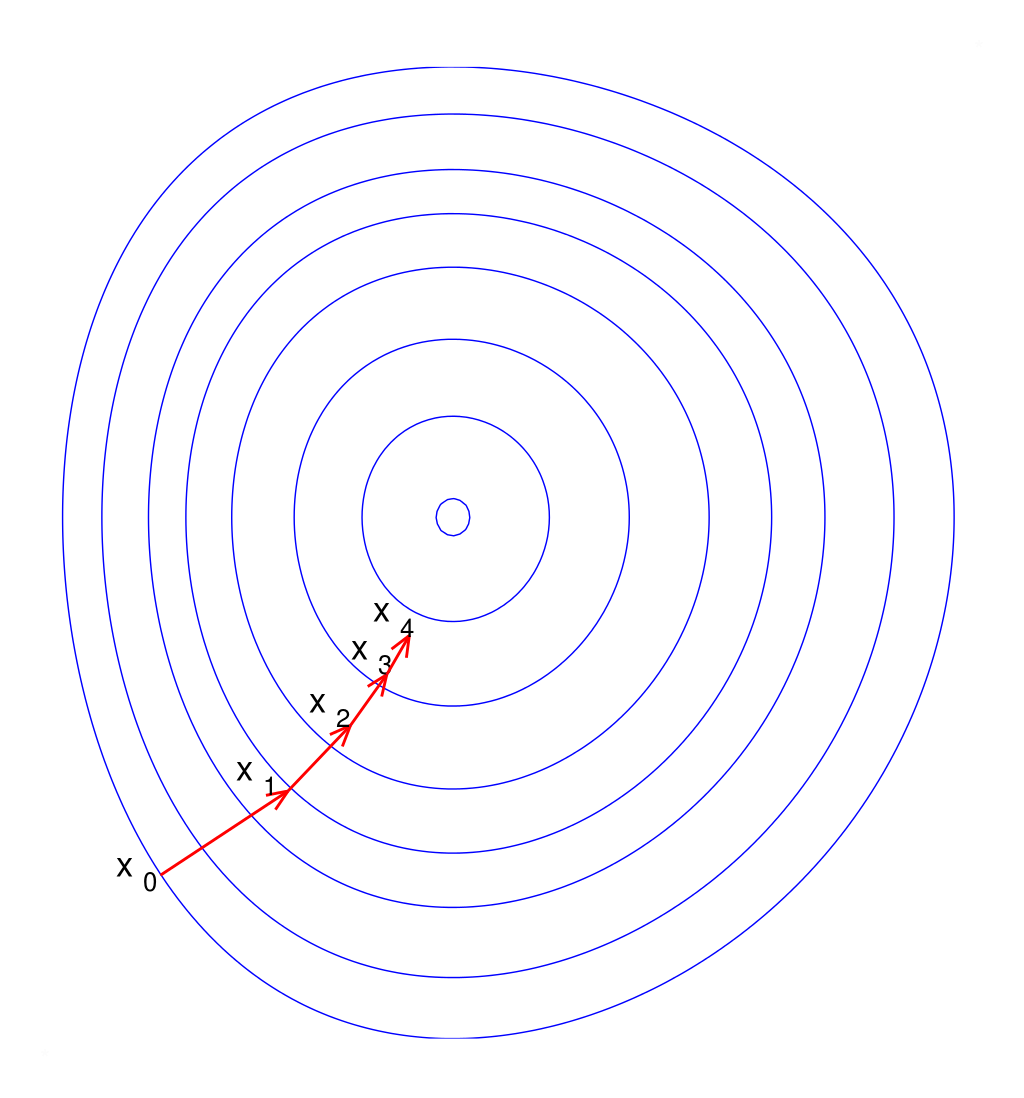
\includegraphics[width=\textwidth]{images/full-gradient-descent.png}
                \end{column}
                \begin{column}{0.5\textwidth}
                    Pros:
                    \begin{itemize}
                        \item This is the true gradient
                        \item You step is guaranteed to yield better performance on all examples
                    \end{itemize}
                    Cons:
                    \begin{itemize}
                        \item It is slow
                        \item You need to run each example before you update any parameters
                    \end{itemize}
                \end{column}
            \end{columns}

            \note{
                \begin{itemize}
                    \item The way we train these models is with something called gradient descent
                    \item This basically means run an example through, calculate how wrong the predicted answer is (the
                        loss), and use the gradient (the derivative) of the parameters with respect to this loss to
                        calculate how to update the parameters.
                    \item In some cases people do full gradient descent where they calculate the answers for each
                        example and get the gradient for everything
                    \item this is good because this is the true gradient, this is the best step you can take to do
                        better next time
                    \item This is slow because you have to weight to run the network on all your data before you update
                        any parameters
                    \item In this picture we can see the big strides in the right direction
                    \item \href{https://commons.wikimedia.org/w/index.php?curid=20569355}{Image from here}
                \end{itemize}
            }
        \end{frame}

        \begin{frame}
            \frametitle{Stochastic Gradient Descent}
            \begin{columns}
                \begin{column}{0.5\textwidth}
                    Pros:
                    \begin{itemize}
                        \item You get to update your parameters each step.
                        \item You can get better generalization because to the randomness.
                    \end{itemize}
                    Cons:
                    \begin{itemize}
                        \item Your gradient could be wrong.
                        \item The gradient for one example can cause a change that is detrimental to another example.
                    \end{itemize}
                \end{column}
                \begin{column}{0.5\textwidth}
                    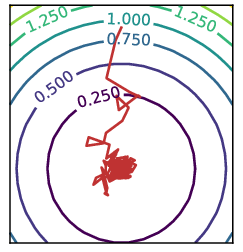
\includegraphics[width=\textwidth]{images/sgd.png}
                \end{column}
            \end{columns}
            \note{
                \begin{itemize}
                    \item On the opposite end of the spectrum we have stochastic gradient descent
                    \item We calculate a gradient and update parameters after each example
                    \item Talk about pros and cons
                    \item In this image we can see how much more random the gradients are
                    \item \href{https://www.researchgate.net/figure/The-two-phase-of-Stochastic-Gradient-Descent-SGD-The-dynamics-consists-of-two-distinct_fig2_315096425}{Image from here}
                \end{itemize}
            }

        \end{frame}

        \begin{frame}
            \frametitle{Mini-Batched Gradient Descent}
            \begin{columns}
                \begin{column}{0.5\textwidth}
                    Pros:
                    \begin{itemize}
                        \item You get to update your parameters more often.
                        \item You can a better approximation of your gradient.
                    \end{itemize}
                \end{column}
                \begin{column}{0.5\textwidth}
                    Cons:
                    \begin{itemize}
                        \item Your need to run the examples in a batch which can be tricky.
                        \item Minibatch size is now a hyperparameter.
                    \end{itemize}
                \end{column}
            \end{columns}
            \note{
                \begin{itemize}
                    \item This is a happy middle ground between the two
                    \item We calculate the gradient for a small batch of examples and update
                    \item Talk about pros and cons
                    \item We can run this mini-batch together via batching
                \end{itemize}
            }
        \end{frame}

        \begin{frame}
            \frametitle{Gradient Accumulation?}
            \begin{itemize}
                \item We saw before that we want to have batches for training dynamics
                \item Why do you have to actually run things at once as a single batch?
                \item Can't you just run each example individually and accumulate the gradients in memory and apply them
                    when you get enough?
                \item Given that I am giving a whole talk on why batching is hard shouldn't you try to avoid it?
            \end{itemize}
            \note{
                \begin{itemize}
                    \item Gradient Accumulation is used when your networks are really large and can't fit on a single
                        GPU
                    \item But we have a good reason to actually batch and that is...
                \end{itemize}
            }
        \end{frame}

        \begin{frame}
            \frametitle{Speed}
            \begin{center}
                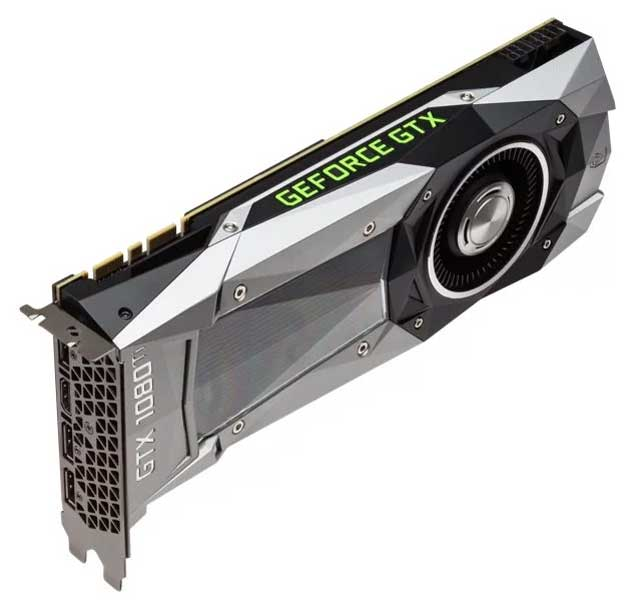
\includegraphics[width=0.7\textwidth]{images/gpu.jpg}
            \end{center}
            \note{
                \begin{itemize}
                    \item
                        \href{https://hothardware.com/news/nvidia-graphics-card-shortage-to-continue-through-q3-2018}{Image
                        from here}
                    \item We showed before that we can express batched operations as matrix matrix multiplications
                    \item Lucky for us humanity has gotten really good at doing these matmuls fast
                    \item We have specialized libraries and even specialized devices like GPUs are designed to do these
                        in a parallel and fast way
                    \item We can stand on the shoulders of gaming to train models really fast
                \end{itemize}
            }
        \end{frame}

    \end{subsection} % Why

\end{section} % Motivation

\begin{section}{Batching is hard in NLP}

    \begin{frame}
        \frametitle{Batching in NLP}

        \begin{itemize}
            \item[]<1-> $$\begin{bmatrix} \text{The} & \text{dog} & \text{ran} & \text{very} & \text{fast} \end{bmatrix}$$
            \item[]<2-> $$\begin{bmatrix} \text{The} & \text{cat} & \text{slept} \end{bmatrix} $$
        \end{itemize}

        \note{
            \begin{itemize}
                \item Now that we know batching is a good idea and you are all really jazzed up about it, I'm going to
                    rain on your parade a bit.
                \item The problem is that batching is pretty hard in NLP
                \item We saw before that batching involves stacking multiple vectors of the same shape into a matrix
                \item In NLP we often have examples that have different lengths
                \begin{itemize}
                    \item Because sentences have different lengths
                    \item Because words have different number of characters in them
                \end{itemize}
                \item We can't just batch any given pair of sentences.
            \end{itemize}
        }
    \end{frame}

    \begin{frame}
        \frametitle{Batching in NLP}

        $$
            \begin{bmatrix}
                \text{The} & \text{dog} & \text{ran} & \text{very} & \text{fast} \\
                \text{The} & \text{cat} & \text{slept} & &
            \end{bmatrix}
        $$
        
\includegraphics[width=\textwidth]{images/x.png}

        \note{
            \begin{itemize}
                \item Here we can't batch these examples because they are different lengths, this would create a ragged
                    array, we need it to be regular.
                \item
                    \href{https://www.kissclipart.com/big-red-x-transparent-background-clipart-desktop-w-3joifc/}{Image
                    from here}
            \end{itemize}
        }
    \end{frame}

    \begin{frame}
        \frametitle{Introducing \textless PAD\textgreater}

        $$
            \begin{bmatrix}
                \text{The} & \text{dog} & \text{ran} & \text{very} & \text{fast} \\
                \text{The} & \text{cat} & \text{slept} & \text{\textless PAD\textgreater} & \text{\textless PAD\textgreater}
            \end{bmatrix}
        $$

        \note{
            \begin{itemize}
                \item Now lets look at how we can handle batching things of different lengths.
                \item We are going to use a new symbol call \textless PAD\textgreater .
                \item We add this to the end of shorter sentence so that all the sentences in a batch have the sample length.
                \item Now that they are all the same length we can turn them into a matrix.
            \end{itemize}
        }
    \end{frame}

    \begin{frame}
        \frametitle{Embeddings and \textless PAD\textgreater}
        \begin{itemize}
            \item In NLP we have an idea of embedding
            \item This is a lookup from word id to a vector representing the word
            \item The principled approach is force the vector for \textless PAD\textgreater \hspace{1pt} to be all zeros
            \item Pytorch \texttt{nn.Embedding} has a \texttt{padding\_idx} parameter that will for the vector with
                    that index to be zero.
            \item Tensorflow you need to role your own.
                \href{https://github.com/dpressel/mead-baseline/blob/f98e64afcbab8a267fce5d13a434a981aa564d27/python/baseline/tf/tfy.py\#L656}{This is an example of doing that in Mead-Baseline}
        \end{itemize}
        \note{
            \begin{itemize}
                \item In general we don't want the network to know anything about the padding
                \item The padding should just be an artifact of batching that doesn't interact with the network or the
                    other values at all
                \item Part of hiding the \textless PAD\textgreater \hspace{1pt} from the network is not letting it learn a
                    representation of the vector
                \item We do this by forcing it to zero
            \end{itemize}
        }
    \end{frame}

    \begin{frame}
        \frametitle{The lengths vector}

        $$
            \begin{bmatrix}
                \text{The} & \text{dog} & \text{ran} & \text{very} & \text{fast} \\
                \text{The} & \text{cat} & \text{slept} & \text{\textless PAD\textgreater} & \text{\textless PAD\textgreater}
            \end{bmatrix}
        $$
        $$
            L = \begin{bmatrix} 5 & 3 \end{bmatrix}
        $$

        \note{
            \begin{itemize}
                \item Now that some of our examples are longer because if this \textless PAD\textgreater we need to track how long the
                    actual data is
                \item We store this in a lengths vector
                \item This will be a vector of the same length as the number of items in the batch
                \item The value will be the number of non padded elements in that example
                \item You can actually have padding on every example in the batch.
                \item This means the length of the physical batch is longer than the maximum value in the lengths vector
                \item This is normally an artifact of being lazy with your data preprocessing, a bit sloppy, and can
                    result in extra computation being done.
                \item Because doing this is wasteful we won't really consider this situation.
            \end{itemize}
        }
    \end{frame}

\end{section} % Hard in NLP

\begin{section}{Batching can Introduce Errors}

    \begin{subsection}{Mean Pooling}
        \begin{frame}
            \frametitle{Mean Pooling}
            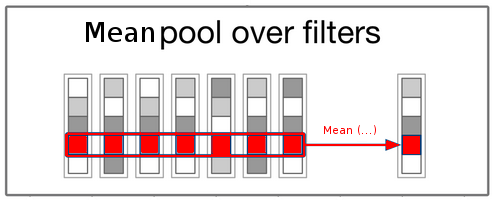
\includegraphics[width=\textwidth]{images/mean-pooling.png}
            \note{
                \begin{itemize}
                    \item As a warm up we are going to look at Mean Pooling.
                    \item The main use-case of mean pooling is in the Neural Bag of Words model.
                    \item We embed each word resulting in a matrix that is sentence length by embedding size
                    \item We do a mean over each time, so each feature is mean-ed separately
                    \item This results in a sentence vector that we can then use for classification
                \end{itemize}
            }
        \end{frame}

        \begin{frame}
            \frametitle{Mean Pooling}
            \begin{itemize}
            \item[]<1->$
                \left[ \begin{array}{*6{c}}
                    1 & 10 & 8 & 17 & 13 & 17
                \end{array} \right] = \frac{66}{6} = 11.0
            $
            \item[]<1->
            \item[]<2->$
                \left[ \begin{array}{*4{c}}
                    22 & 24 & 9 & 13
                \end{array} \right] = \frac{68}{4} = 17.0
            $
            \item[]<3->
            \item[]<3->$
                \left[ \begin{array}{*6{c}}
                    5 & 4 & 8 & 9 & 10 & 34 \\
                    6 & 3 & 1 & 4 & 0 & 0
                \end{array} \right] =
                \left[ \begin{array}{c}
                    \frac{66}{6} \\
                    \frac{68}{6}
                \end{array} \right] =
                \left[ \begin{array}{c}
                    11.0 \\
                    11.\bar{3}
                \end{array} \right]
            $
            \end{itemize}
            \note{
                \begin{itemize}
                    \item Mean pooling gives us a clear example of how padding can get us in trouble
                    \item Side Note: In most of these examples there is actually another dimension of features that
                        these operations are actually acting on but we are going to ignore it and only really look at a
                        single feature in this dimension for simplicity
                    \item Here we see the mean pooling for a vector of length 6
                    \item<2-> Here we see the mean pooling for a length of 4 (shorter)
                    \item<3-> How we see that in order to batch we need to pad the shorter vector
                    \item<3-> Now our denominator is much larger so our result of mean-ing is smaller!
                    \item<3-> Before I said that batching allows us to combine unrelated examples and calculate them in
                        one short and get the same results as if you had calculated them independently
                    \item<3-> When your padding goes wrong the results for an example will be dependent on the other
                        things in the batch. When these padding cases information to bleed across examples this
                        independence is broken and our calculations will be wrong.
                \end{itemize}
            }
        \end{frame}

\begin{frame}[fragile]
    \frametitle{Mean Pooling}

    \begin{pythoncode}
            >>> x
            array([[ 1, 10,  8, 17, 13, 17],
                   [22, 24,  9, 13,  0,  0]])
            >>> np.mean(x, axis=1)
            array([11.        , 11.33333333])
            >>> lengths
            array([6, 4])
            >>> np.sum(x, axis=1) / lengths
            array([11., 17.])
    \end{pythoncode}

    \note{
        \begin{itemize}
            \item We can solve this by explicitly using the lengths vector.
            \item We can manually do our sum and then divide by the actual length instead of the length of the padded
                vector
            \item This assumes that the padded value is zero. Soon we will see how to insure that.
            \item This sort of thing is important because if you don't do it then values will dependent on what else is
                in the batch.
            \item This problem is especially important in training vs production environments
            \begin{itemize}
                \item when training it an example is almost always in a batch
                \item When you are in a batch is is relatively rare to be the longest so being correct in the presence
                    of padding is important
                \item In prod you are often a single example and you are by definition the longest thing in the batch
                \item This means that you need to have the same results with and without padding
            \end{itemize}
        \end{itemize}
    }

\end{frame}

    \end{subsection} % Mean Pooling

    \begin{subsection}{Token Level Losses}
        \begin{frame}
            \frametitle{Cross Entropy}

            \[
                L_{\text{cross-entropy}}(\hat{y}, y) = - \sum_i y_i \log (\hat{y}_i)
            \]
            \note{
                \begin{itemize}
                    \item Out next example of where padding can get up to no good is in our loss functions
                    \item Our normal loss is the cross entropy loss between two vectors
                    \item $y$ is the vector that has a our labels and $\hat{y}$ is out predicted labels
                    \item cross entropy is a measure of the difference between two distributions
                    \item The cross entropy is the sum of the true value times the log of the predicted values
                    \item In classifiction where we output a probability distribution over classes we can use this loss
                        function to train the model
                \end{itemize}
            }
        \end{frame}

        \begin{frame}
            \frametitle{Sparse Cross Entropy}

            \[
                L_{\text{cross-entropy}}(\hat{y}, y) = - \sum_i y_i \log (\hat{y}_i)
            \]
            \[
                L_{\text{sparse-cross-entropy}}(\hat{y}, y) = - \log(\hat{y_i}[y])
            \]
            \note{
                \begin{itemize}
                    \item Because our labels are always a one hot vector (it only has a 1 at the location that represents
                        the label index) most of these elements in this sum will be zero
                    \item In fact the only value will be the probability for the predicted class
                    \item We can short cut this calculation by just indexing the predicted vector with the true class
                        index
                    \item This is what we call sparse cross entropy
                \end{itemize}
            }
        \end{frame}

        \begin{frame}<1>
            \frametitle{Token-Level (Sparse) Cross Entropy Loss}
            \begin{align*}
                T &\coloneqq \text{length of example} \\
                V &\coloneqq \text{number of possible labels} \\
                s &\in \R^{T \text{ x } V} \\
                l &\in \N^T \\
                J &= - \sum_{i}^{T} s_i[l_i] \\
            \end{align*}

            \note{
                \begin{itemize}
                    \item This idea of sparse cross entropy can be extend to the idea of a token level loss.
                    \item This means that a decision is made for every token and we calculate the loss for the
                        probability vector that is output for each token in a sentence.
                    \item We will see soon how this loss at the padding positions can mess us up.
                    \item Here we see the cross entropy loss where we have a matrix of scores. Each row represents the
                        scores of a token and each column is the score for some class.
                    \item Our loss is then the sum (or mean) of the score for each token.
                    \item This kind of loss is often used for language modeling where the label is the index of the next
                        word or else sequence tagging where the label is the tokens tag.
                \end{itemize}
            }
        \end{frame}

        \begin{frame}
            \frametitle{(Sparse) Cross Entropy Loss}
            \begin{align*}
                s &= \left[ \begin{array}{*5{c}}
                    -0.34 & 0.1 & -0.11 & \cdots & 0.001 \\
                    0.93 & -8.88 & -0.39 & \cdots & 0.12 \\
                    & & \vdots & & \\
                    -0.45 & 0.23 & 1.1 & \cdots & -0.3
                \end{array} \right] \\
                l &= \left[ \begin{array}{*5{c}}
                    2 & 1 & 10 & 5 & 1
                \end{array} \right] \\
                J &= \left[ \begin{array}{*5{c}}
                    -0.11 & -8.88 & 0.28 & 0.43 & 0.23
                \end{array} \right]
            \end{align*}
            \note{
                \begin{itemize}
                    \item Here we see some examples of score, labels, and the selected scores.
                \end{itemize}
            }
        \end{frame}

        \begin{frame}
            \frametitle{(Sparse) Cross Entropy Loss}
            \begin{align*}
                s &= \left[ \begin{array}{*5{c}}
                    -0.34 & 0.1 & -0.11 & \cdots & 0.001 \\
                    0.93 & -8.88 & -0.39 & \cdots & 0.12 \\
                    & & \vdots & & \\
                    -0.45 & 0.23 & 1.1 & \cdots & -0.3
                \end{array} \right] \\
                l &= \left[ \begin{array}{*5{c}}
                    2 & 1 & 10 & 5 & 1 \\
                    5 & 6 & 3 & &
                \end{array} \right] \\
                J &= \left[ \begin{array}{*5{c}}
                    -0.11 & -8.88 & 0.28 & 0.43 & 0.23 \\
                    -3.4 & 0.6 & 0.37 & -956.0 & 10000.0
                \end{array} \right]
            \end{align*}
            \note{
                \begin{itemize}
                    \item Here we see what can happen when you are batching and have a shorter sentence.
                    \item When you are selecting the scores for the padding tokens they really could be anything
                    \item We don't really want the network to have to learn to output a padding symbol after the normal
                        length, that isn't a situation you would really have a use for.
                    \item We also don't want random lucky values to make our loss look really good.
                    \item We need a way to zero our the effects of these padded locations
                \end{itemize}
            }
        \end{frame}

\begin{frame}[fragile]
    \frametitle{Making a Mask}
    \begin{pythoncode}
        >>> lengths = np.array([5, 3, 4])
        >>> steps = np.arange(np.max(lengths))
        >>> steps
        array([0, 1, 2, 3, 4])
        >>> mask = (np.reshape(lengths, (-1, 1)) > steps).astype(np.int32)
        >>> mask
        array([[1, 1, 1, 1, 1],
               [1, 1, 1, 0, 0],
               [1, 1, 1, 1, 0]], dtype=int32)
    \end{pythoncode}
    \note{
        \begin{itemize}
            \item We will zero out these values by using a mask
            \item This mask has ones where the valid tokens are and a zero where the padding tokens are.
            \item Here we see how to create a mask.
            \item We create this with broadcasting.
            \item We create a vector of incrementing steps along the dimension that includes padding and compare them to
                the lengths vector.
            \item When the length is longer than the current steps we are still valid so the value is one.
            \item Once the step is longer than the length we are in the pad and will output zeros.
        \end{itemize}
    }
\end{frame}

        \begin{frame}
            \frametitle{(Sparse) Cross Entropy Loss}
            \begin{align*}
                J &= \left[ \begin{array}{*5{c}}
                    -0.11 & -8.88 & 0.28 & 0.43 & 0.23 \\
                    -3.4 & 0.6 & 0.37 & -956.0 & 10000.0
                \end{array} \right]\\
                \text{mask} &= \left[ \begin{array}{*5{c}}
                    1 & 1 & 1 & 1 & 1 \\
                    1 & 1 & 1 & 0 & 0
                \end{array} \right] \\
                J * \text{mask} &= \left[ \begin{array}{*5{c}}
                    -0.11 & -8.88 & 0.28 & 0.43 & 0.23 \\
                    -3.4 & 0.6 & 0.37 & 0 & 0
                \end{array} \right]\\
            \end{align*}
            \note{
                \begin{itemize}
                    \item Here we can use our mask to force the padding locations to zero.
                    \item We can then sum the values (or mean them with the lengths if you want).
                    \item Some toolkits like Pytorch can handle this for you, you give a value to the
                        \texttt{padding\_idx} parameter and it will ignore values where the label is that padding index
                    \item Toolkits like tensorflow will probably make you do this our self.
                \end{itemize}
            }
        \end{frame}

    \end{subsection} % Token Level Losses

    \begin{subsection}{Attention}

        \begin{frame}
            \frametitle{Attention}
            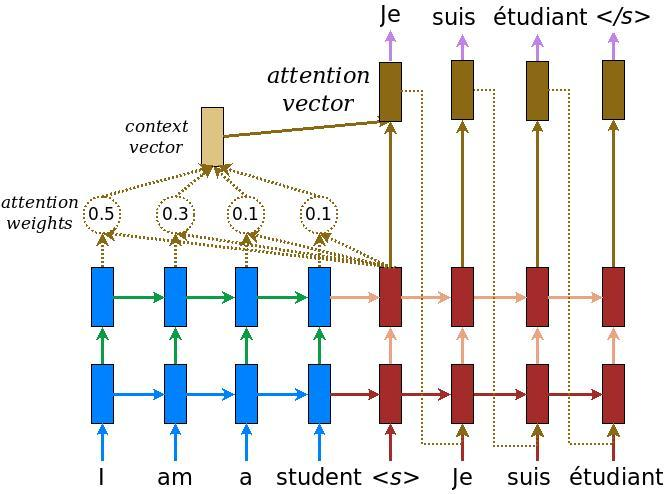
\includegraphics[width=\textwidth]{images/attention.jpg}
            \note[size=\tiny]{
                \begin{itemize}
                    \item Attention is used to contextualize a vector relative to others.
                    \item We have some vector here in the decoder and want to create a new vector that summarizes the
                        information in these vectors created by the encoder that is relevant to decoder vector.
                    \item We do this by creating a similarity score between the vector we care about and each vector in
                        the memory bank of vectors
                    \item We then normalize these values and create new vector by taking a weight average of the memory
                        bank
                    \item This is often used in seq2seq models to short cut information from the encoder into the
                        decoder
                    \item \href{https://www.tensorflow.org/tutorials/text/nmt_with_attention}{Image From Here}
                \end{itemize}
            }
        \end{frame}

        \begin{frame}
            \frametitle{Attention}
            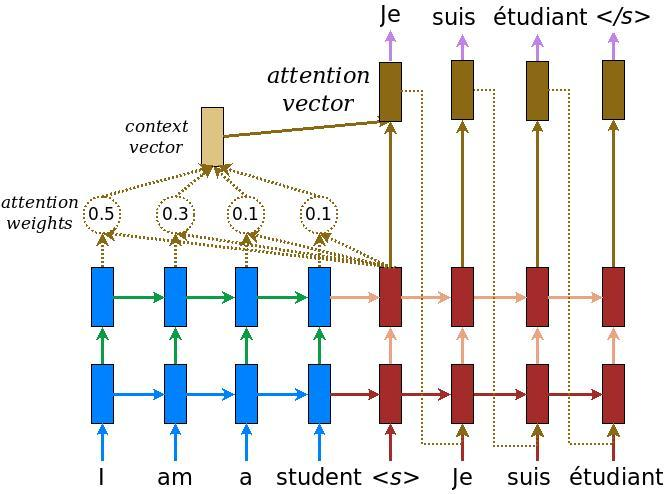
\includegraphics[width=\textwidth]{images/attention.jpg}
            \note[size=\tiny]{
                \begin{itemize}
                    \item In a more general format we have 3 sets of vectors
                    \begin{itemize}
                        \item Query Vectors: the ones we are processing right now
                        \item Key Vectors: The ones we are doing the similarity score with
                        \item Value Vectors: The ones that are actually mixed together
                    \end{itemize}
                    \item In some cases these vectors can be the same (for example RNN Seq2seq normally use $K = Q$) in
                        other case they are either different or the same thing projected into different spaces
                    \item The point of this is that the representation of a vector that is useful down stream might not
                        be one that is similar to the query vectors so the keys can be the similar ones.
                    \item \href{https://www.tensorflow.org/tutorials/text/nmt_with_attention}{Image From Here}
                \end{itemize}
            }
        \end{frame}

        \begin{frame}
            \frametitle{Attention}

            \begin{align*}
                q &= \begin{bmatrix}
                    \text{---} & q & \text{---}
                    \end{bmatrix} \\
                K &= \begin{bmatrix}
                         \vert & \vert & & \vert \\
                         k_1 & k_2 & \cdots & k_n \\
                         \vert & \vert & & \vert
                     \end{bmatrix} \\
                s &= \similar(q, K) = \begin{bmatrix}
                        s_1 & s_2 & \cdots & s_n \\
                    \end{bmatrix}
            \end{align*}

            \note{
                \begin{itemize}
                    \item First we calculate a score between the vectors
                    \item There are multiple ways to calculate these similarities, the original paper used a small
                        neural network, later architectures (notably the transformer) use the dot product to calculate
                        the score.
                    \item The transformer actually uses the scaled dot product where it divides the score by $\sqrt{d_k}$
                        because the dot product will get larger as the vectors get larger
                    \item In this case we are just using a single vector for $q$ but we can actually use a matrix $Q$ to
                        calculate the attention between multiple vectors at once.
                    \item This vector version is common for RNN seq2seq models (where you have single vector at each timestep)
                    \item The Matrix version is used in the transformer where we want to do attention for the whole sentence at once
                \end{itemize}
            }
        \end{frame}

        \begin{frame}
            \frametitle{Attention}
            \begin{align*}
                s &= \similar(q, K) = \begin{bmatrix}
                        0.21 & -0.34 & \cdots & 0.55 \\
                    \end{bmatrix} \\
                \softmax(x) &= \frac{e^{x_i}}{\sum_j e^{x_j}} \\
                \alpha &= \softmax(s) = \begin{bmatrix}
                        0.1684 & 0.0977 & \cdots & 0.2379 \\
                    \end{bmatrix} \\
            \end{align*}

            \href{https://blester125.com/blog/softamx.html}{Numerically stable softmax blog post.}
            \note{
                \begin{itemize}
                    \item Then we use the softmax so the score are all positive and they sum to one.
                    \item The softmax is the done by exponentiating each element and then normalizing the elements.
                    \item I have a blog post about how you can do that in a numerically stable way if you decide to roll
                        your own implementation.
                    \item We can then uses these scores to do a weight average.
                \end{itemize}
            }
        \end{frame}

        \begin{frame}
            \frametitle{Attention}
            \begin{align*}
                V &= \begin{bmatrix}
                         \vert & \vert & & \vert \\
                         v_1 & v_2 & \cdots & v_n \\
                         \vert & \vert & & \vert
                     \end{bmatrix} \\
                s &= \similar(q, K) = \begin{bmatrix}
                        s_1 & s_2 & \cdots & s_n \\
                    \end{bmatrix} \\
                \alpha &= \softmax(s) \\
                c &= V * \alpha^{T} \\
            \end{align*}
            \note{
                \begin{itemize}
                    \item Then we do a weighted average of the value vectors based on these calculated (and normalized) scores.
                    \item Now $c$ is a combination of the vectors in $V$ weighted by their attention scores which were
                        calculated based on the similarity of the query vectors to $q$
                \end{itemize}
            }
        \end{frame}

        \begin{frame}
            \frametitle{Attention}

            \begin{align*}
                K &= \begin{bmatrix}
                        \vert & \vert & & \vert & \vert \\
                        k_1 & k_2 & \cdots & \text{\textless PAD\textgreater} & \text{\textless PAD\textgreater} \\
                        \vert & \vert & & \vert & \vert \\
                     \end{bmatrix} \\
                s &= \begin{bmatrix}
                        s_1 & s_2 & \cdots & 0 & 0
                     \end{bmatrix}
            \end{align*}

            \note{
                \begin{itemize}
                    \item But what happens when we calculate the similarity between vectors that have padding on them?
                    \item With most similarity metrics (dot/scaled dot product) we do get zeros for the similarity between
                        a padding vector and a valid vector (assuming the pad is zeros)
                    \item Is this enough so that our calculations will be correct?
                    \item Would I have brought this up if it was?
                \end{itemize}
            }
        \end{frame}

\begin{frame}[fragile]
    \frametitle{Attention}
    \begin{pythoncode}
  >>> x = np.array([
          [0.32, 0.11, 0.83, 0.9, 0.4],
          [0.5, 0.2, -1.0, 0, 0]
      ])
  >>> x
  array([[ 0.32,  0.11,  0.83,  0.9 ,  0.4 ],
         [ 0.5 ,  0.2 , -1.  ,  0.  ,  0.  ]])
  >>> softmax(x)
  array([[0.15759942, 0.12774761, 0.26244893, 0.28147862, 0.17072542],
         [0.31476139, 0.23318098, 0.07023276, 0.19091244, 0.19091244]])
    \end{pythoncode}
    \note{
        \begin{itemize}
            \item Here we can see that when the scores going into the softmax are zero we will get non-zero scores out!
            \item This means that when we do the mixing of the value vectors were are going to include the padding
                vectors in our weighted average.
            \item What we need to have there be zeros \textbf{after} the softmax which will zero out the contribution of
                the padding.
        \end{itemize}
    }
\end{frame}

\begin{frame}[fragile]
    \frametitle{Attention}
    \begin{pythoncode}
  >>> mask = make_mask(np.array([5, 3]))
  >>> mask
  array([[1, 1, 1, 1, 1],
         [1, 1, 1, 0, 0]], dtype=uint8)
  >>> attn = softmax(x) * mask
  >>> attn
  array([[0.15759942, 0.12774761, 0.26244893, 0.28147862, 0.17072542],
         [0.31476139, 0.23318098, 0.07023276, 0.        , 0.        ]])
  >>> np.sum(attn, axis=1)
  array([1.        , 0.61817513])
  >>> softmax(x[1:np.newaxis, 0:3])
  >>> array([[0.50917835, 0.3772086 , 0.11361305]])
    \end{pythoncode}
    \note{
        \begin{itemize}
            \item Ok, our first cut is just masking out those padding weights, now their values are zero so they won't 
                contribute to the weighted average anymore.
            \item Is this ok?
            \item We can see that the values for this example don't sum to one any more, this solution isn't enough
            \item We we can also see that the values calculated for the sorter batch are very different then when that
                example is calculated by itself.
            \item Remember the whole point of batching is that we should be able to run multiple examples at once
                and get the same values as if we ran them through one at a time
        \end{itemize}
    }
\end{frame}

\begin{frame}[fragile]
    \frametitle{Attention}
    \begin{pythoncode}
  >>> inv_mask = (1 - mask) * -1e9
  >>> masked_x = (x * mask) + inv_mask
  >>> masked_x
  array([[ 3.2e-01,  1.1e-01,  8.3e-01,  9.0e-01,  4.0e-01],
         [ 5.0e-01,  2.0e-01, -1.0e+00, -1.0e+09, -1.0e+09]])
  >>> softmax(masked_x)
  array([[0.15759942, 0.12774761, 0.26244893, 0.28147862, 0.17072542],
         [0.50917835, 0.3772086 , 0.11361305, 0.        , 0.        ]])
  >>> softmax(x[1:np.newaxis, 0:3])
  >>> array([[0.50917835, 0.3772086 , 0.11361305]])
  >>> softmax(masked_x).sum(axis=1)
  array([1., 1.])
    \end{pythoncode}
    \note[size=\tiny]{
        \begin{itemize}
            \item We need to hack softmax to force it to output zeros for the padded values while the other values sum
                to one.
            \item We know that the softmax will exponentiate each element and we know that exponentiation by a negative
                number of will approach zero as the exponent grows.
            \item With a sufficiently negative number we can force an element to zero
            \item On this first line \texttt{(1 - mask)} will flip a mask of ones and zeros.
            \begin{itemize}
                \item $1 - 1 = 0$ and $1 - 0 = 1$
                \item This will mean that the ones are now where the pads and zero where the valid elements are
            \end{itemize}
            \item Then we multiply in a very negative number so out mask is all zeros and this neg
            \item We multiply by the mask to make sure the padding locations are zero (not strictly necessary) then we
                add the inverse mask in.
            \item the inverse mask has all zeros for the valid elements so they don't change but it has $-1e^9$ for the
                pad so zero + that negative is that negative
            \item Now when we do the softmax we see that out values match and they sum to one in each axis
        \end{itemize}
    }
\end{frame}

        \begin{frame}
            \frametitle{Attention}

            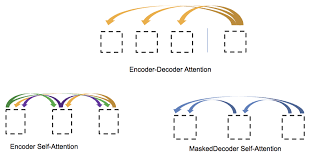
\includegraphics[width=\textwidth]{images/self-attention.png}

            \note{
                \begin{itemize}
                    \item We have been looking at encoder-decoder attention where we compare a vector in the decoder to
                        the values in the encoder.
                    \item There is also self attention were we compare to all the tokens around us.
                    \item There is also a special case of self attention where we can use a mask to enforce causality
                    \item This mask would stop the attention from looking forward in time at words that haven't been
                        generated yet.
                    \item This mask works the same way as the length mask.
                    \item Some times you need to combine these masks.
                    \item Attention is an example where just masking out the padding value isn't enough, we actually have to
                        manipulate the padding values in a specific way.
                    \item
                        \href{https://web.stanford.edu/class/archive/cs/cs224n/cs224n.1184/lectures/lecture12.pdf}{Image
                        is from here}
                \end{itemize}
            }
        \end{frame}

    \end{subsection} % Attention

    \begin{subsection}{Conditional Random Field}

        \begin{frame}
            \frametitle{Conditional Random Field}

            \begin{center}
                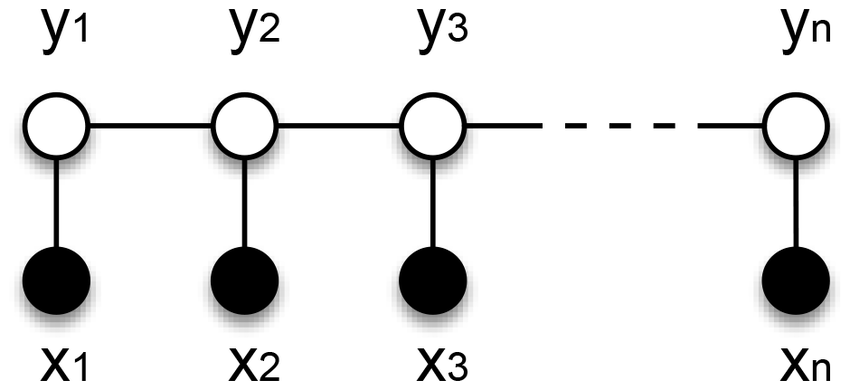
\includegraphics[width=0.6\textwidth]{images/crf.png}
            \end{center}
            $$
                P(y|x;\theta) = \frac{\exp(\sum_i \sum_j w_j f_j(y_{i-1}, y_i, x, i))}{\sum_{y' \in Y}\exp(\sum_i
                \sum_j w_j f_j(y'_{i - 1}, y'_i, x i))}
            $$
            \begin{center}
                \href{https://createmomo.github.io/2017/09/12/CRF_Layer_on_the_Top_of_BiLSTM_1/}{Great Tutorial on CRFs}
            \end{center}

            \note{
                \begin{itemize}
                    \item This is our most complex example so it is ok if you don't understand everything
                    \item In our token level loss from before we made decision about the label of a token without
                        considering the label we chose for the last one.
                    \item Here is this factor graph diagram of a CRF we see that the label decisions are conditioned on
                        the previous label. This makes the CRF a global model.
                    \item In the token level loss our scores and therefore the label decision were contextual in that
                        they were based on the whole input (from an RNN or something) but they don't consider the past
                        labels so it doesn't have any idea of global coherence.
                    \item These scores are called the local representation of the token.
                    \item A trend in research is to buff these local representations while not caring about the global
                        part to much
                    \item Problems that deal with making a sequence of decisions like are called structured
                        prediction problems
                    \item
                        \href{https://www.researchgate.net/figure/Linear-chain-conditional-random-fields-model-Black-nodes-represent-observable-values_fig20_263324470}{Image
                        from Here}
                \end{itemize}
            }
        \end{frame}

        \begin{frame}
            \frametitle{Conditional Random Field}

            \begin{center}
                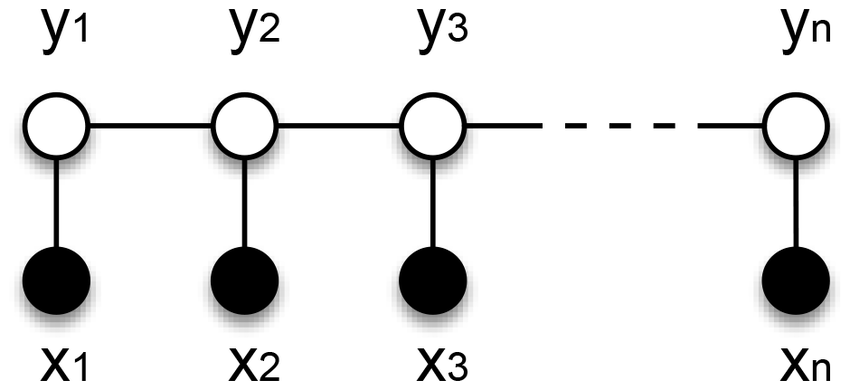
\includegraphics[width=0.6\textwidth]{images/crf.png}
            \end{center}
            $$
                P(y|x;\theta) = \frac{\exp(\sum_i \sum_j w_j f_j(y_{i-1}, y_i, x, i))}{\sum_{y' \in Y}\exp(\sum_i
                \sum_j w_j f_j(y'_{i - 1}, y'_i, x i))}
            $$
            \begin{center}
                \href{https://createmomo.github.io/2017/09/12/CRF_Layer_on_the_Top_of_BiLSTM_1/}{Great Tutorial on CRFs}
            \end{center}

            \note{
                \begin{itemize}
                    \item Our loss function here can help illustrate the differences
                    \item Thinking back to our token level loss function our loss was the sum of the losses at each step
                    \item This is explicitly optimizing this local decision making process.
                    \item In this loss function we see that we are actually acting on the sequence level
                    \item Our loss is now the score you model gives the gold sequence $y$
                    \item Normalized but the score of the possible sequences.
                    \item We want to optimize it so more probability is placed on the gold sentence
                    \item
                        \href{https://www.researchgate.net/figure/Linear-chain-conditional-random-fields-model-Black-nodes-represent-observable-values_fig20_263324470}{Image
                        from Here}
                \end{itemize}
            }
        \end{frame}

        \begin{frame}
            \frametitle{Conditional Random Field - Best Path}
            \begin{align*}
                t &\coloneqq \text{number of tokens} \\
                c &\coloneqq \text{number of classes} \\
                e &\in \R^{t \text{ x } c} \\
                t &\in \R^{c \text{ x } c} \\
                y &\in \N^t \\
                \text{gold score} &= \sum_i e_i[y_i] + t[y_{i - 1}, y_i]
            \end{align*}
            \note{
                \begin{itemize}
                    \item $e$ is our emission scores, this tells us the class scores for each token. This is the local
                        representation of the token
                    \begin{itemize}
                        \item One thing to note is that these scores are unnormalized (not softmaxed). This lets us
                            avoid some problems locally normalized models have but that is out of scope
                    \end{itemize}
                    \item $t$ is our transition scores, this tells us the score of moving from one class to another at
                        the next step.
                    \item $e$ is a score tensor that is output by the network whereas $t$ is a parameter that is learned
                    \item Our score is sum over tokens of emission score for that label plus the score of transitioning
                        to that label from the previous label.
                    \item It is easy to see how if you have padding you are going to get junk in your score, The
                        emission score and the transistors involving padding will get in there
                    \item This is an easy fix we have seen before, before you sum across the tokens use your mask to set
                        the padding values to zero and you'll get the right score.
                \end{itemize}
            }
        \end{frame}

        \begin{frame}
            \frametitle{Conditional Random Field - All Paths}
            \begin{align*}
                t &\coloneqq \text{number of tokens} \\
                c &\coloneqq \text{number of classes} \\
                \alpha &\in \R^S \\
                e &\in \R^{t \text{ x } c} \\
                t &\in \R^{c \text{ x } c} \\
                \forall_{i \in t} \hspace{2pt} \alpha_i &= \logsumexp(\alpha_{i - 1} + e_i^T + t) \\
            \end{align*}
            \note{
                \begin{itemize}
                    \item When calculating all paths you can't actually enumerate all the possible paths. There are
                        $t^c$ possible paths.
                    \item We can use a dynamic programming to do this, it is out of scope though.
                    \item We have $\alpha$ which represents the total score for any path that ends up in this label
                    \item We often initialize this $\alpha$ with all the score on a fake \textless START\textgreater
                        \hspace{1pt} that helps us represent which labels often start a sequence.
                    \item We calculate a new version of these scores at each time step and overwrite the previous
                        $\alpha$s
                    \item We need to make sure that we only update the $\alpha$ if we are transitioning to a valid token
                    \item If we are looking at a \textless PAD\textgreater \hspace{1pt} we don't want to update the
                        alpha.
                \end{itemize}
            }
        \end{frame}

        \begin{frame}
            \frametitle{Conditional Random Field - All Paths}
            \begin{algorithm}[H]
                % \SetAlgoLined
                $T \coloneqq \text{number of tokens in batch}$\;
                $c \coloneqq \text{number of classes}$\;
                $t \coloneqq \text{number of valid tokens in example}$\;
                $\alpha \in \R^S$\;
                $e \in \R^{t \text{ x } c}$\;
                $t \in \R^{c \text{ x } c}$\;
                \For{$i \gets 0$ \KwTo $T$}{
                    \eIf{$i < t$}{
                        $\alpha = \logsumexp(\alpha + e_i^T + t)$\;
                    }{
                        $\alpha = \alpha$
                    }
                }
            \caption{The Forward Algorithm}
            \end{algorithm}
            \note{
                \begin{itemize}
                    \item I have removed the \textless START \textgreater \hspace{2pt} and \textless END \textgreater
                        \hspace{2pt} from this algorithm but you should use them, they are a higher-fidelity
                        representation and let you model which starts the likely to start of end a sequence
                    \item This boils down to a simple conditional.
                    \item If we are still inside the valid tokens we assign alpha based on the results of the dynamic
                        programming algorithm
                    \item If we are in the padding step we just reuse the old $\alpha$s
                    \item How do we implement this conditional with masking?
                \end{itemize}
            }
        \end{frame}

\begin{frame}[fragile]
    \frametitle{Conditional Random Field}
    \begin{pythoncode}
>>> lengths = np.array([3, 1, 5])
>>> lengths
array([3, 1, 5])
>>> for i in range(np.max(lengths)):
...     new_alphas = calculate_step(alpha, emission, transition, i)
...     mask = (i < lengths).astype(np.uint8)
...     print(mask)
...     alphas = (alpha * mask) + (new_alphas * (1 - mask))
[1 1 1]
[1 0 1]
[1 0 1]
[0 0 1]
[0 0 1]
    \end{pythoncode}
    \note{
        \begin{itemize}
            \item In this example we can see how we can use create masks that represent conditionals.
            \item First we track how far we are into the loop with the $i$ variable.
            \item First we calculate the updated alphas regardless of whether we are padding or not
            \item Then we make a mask where we have ones if we are inside the valid lengths
            \item Then we update the alphas based on the mask so that we only update the ones we should.
        \end{itemize}
    }
\end{frame}

\begin{frame}[fragile]
    \frametitle{Conditional Random Field}
    \begin{pythoncode}
        >>> a
        array([1, 2, 3, 4, 5])
        >>> b
        array([-1, -2, -3, -4, -5])
        >>> mask = np.where(a >= 4, 1, 0)
        >>> mask
        array([0, 0, 0, 1, 1])
        >>> (a * mask) + (b * (1 - mask))
        array([-1, -2, -3,  4,  5])
    \end{pythoncode}
    \note{
        \begin{itemize}
            \item This is a more illustrative example.
            \item We see positive and negative values.
            \item We make a mask that represents ``if $a >= 4$ then return $a$ else return $b$''.
            \item We multiply $a$ by the mask so now all the values are zero when the conditional is false.
            \item We multiply $b$ by the inverse mask, this makes the elements where $a$ is non zero 0.
            \item No the non-zero values are disjoint between $a$ and $b$.
            \item We add the vectors to combine the results.
        \end{itemize}
    }
\end{frame}

        \begin{frame}
            \frametitle{Conditional Random Field}
            \begin{center}
                A complex layer with complex padding \\
                \vspace{10pt}
                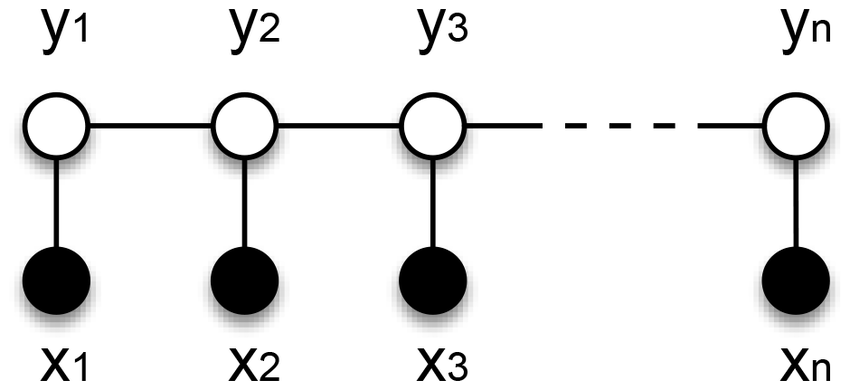
\includegraphics[width=0.6\textwidth]{images/crf.png}
            \end{center}
            \note{
                \begin{itemize}
                    \item The CRF is a rather complex layer but the main reason I brought it up here is that it introduces a new way
                        that we need to handle padding.
                    \item We are using the mask to simulate a conditional.
                    \item This is common in parallel processing where we compute both branches of a conditional and use
                        a mask to combine the result according to that conditional.
                \end{itemize}
            }
        \end{frame}

        \begin{frame}
            \frametitle{Viterbi}

            \begin{itemize}
                \item When we predict actual tags from a CRF we use the Viterbi algorithm to find the maximum scoring
                    path.
                \item The algorithm is the exact same as the forward algorithm except that use us a $\max$ instead of a
                    $\logsumexp$ when computing the new $\alphas$
                \item $\alpha$ now represents the maximum score of any path that ends at each class
                \item We can using the exact same padding trick when doing Viterbi decoding!
            \end{itemize}
            \note{
                \begin{itemize}
                    \item A way to look at these two algorithms is that they are the same algorithm using different
                        semirings. We basically define different operations for sums and additions
                        \begin{itemize}
                            \item The CRF forward is on the log semiring where the addition is a log sum exp addition
                            \item The Viterbi algorithm is on the Viterbi semiring where the addition is a maximum
                        \end{itemize}
                    \item in the CRF $\alpha$ was the sum of scores for all paths that end in some class
                    \item in Viterbi $\alpha$ is the maximum score of any path that ends in some class
                \end{itemize}
            }
        \end{frame}

        \begin{frame}
            \frametitle{Viterbi - Getting a Path}

            \begin{center}
                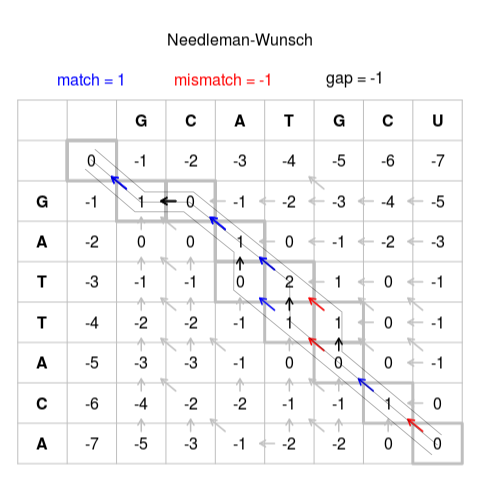
\includegraphics[width=0.7\textwidth]{images/backtrack.png}
            \end{center}

            \note{
                \begin{itemize}
                    \item Like most dynamic programming algorithms you need to store your decisions so you can back
                        track through to get your actual answer
                    \item In this picture we can see these arrows that tell us where we came from and can be used to
                        recover the edit path.
                    \item When doing Viterbi decoding we calculate these backtracks with the argmax
                    \item As we calculate the back tracking we need to not overwrite the final decision once we hit the
                        end of the valid lengths
                    \item We use the same kind of padding we used above for this.
                    \item When we are following the backtrack we need to do something similar but flip the lengths we
                        care about because we are reading from the back of the tensor.
                    \item \href{https://en.wikipedia.org/wiki/Needleman\%E2\%80\%93Wunsch_algorithm}{Image from here}
                    \item Now that we have talked about some complex cases lets look at some subtle ones.
                \end{itemize}
            }
        \end{frame}

    \end{subsection} % CRF

    \begin{subsection}{Max Pooling}

        \begin{frame}
            \frametitle{Max Pooling}
            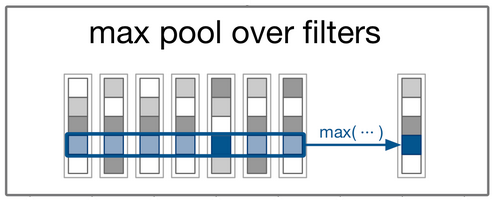
\includegraphics[width=\textwidth]{images/mot-pooling.png}
            \note{
                \begin{itemize}
                    \item Max pooling is often applied across a feature dimension in the same way that mean pooling is
                    \item Here we see a set of vectors, each one is a featured representation of a word in a sentence
                    \item We do max pooling across a single feature dimension.
                    \item We end up with a single vector where each feature is the largest value that feature took in
                        the course of the sentence
                    \item We can also do this at a word level where each vector represents a character in a word
                    \item A common use case is to encode words with a Convolutional Network (which we will get to soon)
                        and then aggregate the results with max pooling.
                    \item \href{https://jessicastringham.net/2018/12/30/conv-max-pool/}{Image from here}
                \end{itemize}
            }
        \end{frame}

        \begin{frame}
            \frametitle{Max Pooling}
            \begin{align*}
                x &= \begin{bmatrix}
                    1 & 0 & 4 & 3 & 2 & 0 & 0
                \end{bmatrix}\\
                \text{lengths} &= \begin{bmatrix} 5 \end{bmatrix} \\
                \max(x) &= 4
            \end{align*}
            \note{
                \begin{itemize}
                    \item Here we are zoomed in a single feature over time, these are the numbers in the blue
                        highlighted area on the last slide
                    \item Lets say these vectors we are zoomed in one just went through a ReLU $\max(0, x)$ so it will
                        never have a negative number in it.
                    \item This example has a length of 5 which means the last two zero features are padding
                    \item Pop Quiz: Is it safe to do a max without thinking about padding?
                    \item \textbf{YES}
                \end{itemize}
            }
        \end{frame}

        \begin{frame}
            \frametitle{Max Pooling}
            \begin{align*}
                x &= \begin{bmatrix}
                    -3 & -1 & -4 & -3 & -2 & 0 & 0
                \end{bmatrix}\\
                \text{lengths} &= \begin{bmatrix} 5 \end{bmatrix} \\
                \max(x) &= 0 \\
                \max(x[:5]) &= -1
            \end{align*}
            \note{
                \begin{itemize}
                    \item What about a vector that looks like this?
                    \item Lets say here we are looking at a feature of a word right after embedding.
                    \item Your max pooling it going to output zero for this feature!
                    \item Your network will never see a negative value for most examples while training! (most examples
                        are padded)
                    \item Your network will see these negative values at test time and have no idea what to do!
                    \item How do we fix this?
                \end{itemize}
            }
        \end{frame}

        \begin{frame}
            \frametitle{Max Pooling}
            \begin{align*}
                x' &= \begin{bmatrix}
                    -3 & -1 & -4 & -3 & -2 & -10000 & -10000
                \end{bmatrix}\\
                \text{lengths} &= \begin{bmatrix} 5 \end{bmatrix} \\
                \max(x') &= -1
            \end{align*}
            \note{
                \begin{itemize}
                    \item We use the same trick we used in attention, by setting the pads so a very negative value we
                        can ensure they will never be picked
                \end{itemize}
            }
        \end{frame}

        \begin{frame}
            \frametitle{Min Pooling}
            \begin{align*}
                x &= \begin{bmatrix}
                    3 & 1 & 4 & 3 & 2 & 0 & 0
                \end{bmatrix}\\
                x' &= \begin{bmatrix}
                    3 & 1 & 4 & 3 & 2 & 10000 & 10000
                \end{bmatrix}\\
                \text{lengths} &= \begin{bmatrix} 5 \end{bmatrix} \\
                \min(x) &= 0 \\
                \min(x[:5]) &= 1\\
                \min(x') &= 1
            \end{align*}
            \note{
                \begin{itemize}
                    \item This same thing applies in Min pooling, we where the padding can be selected as the minimum.
                    \item We can solve this similarly but set the padding to a very high value.
                \end{itemize}
            }
        \end{frame}

    \end{subsection} % Max Pooling

    \begin{subsection}{Convolution 1D}

        \begin{frame}
            \frametitle{Convolution 1D}
            \begin{center}
                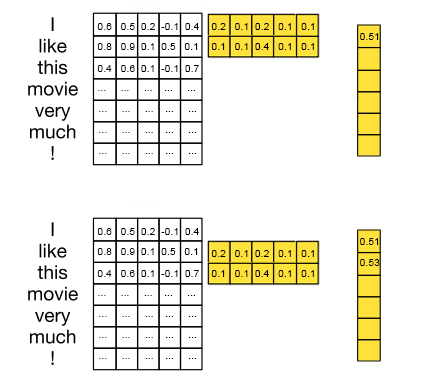
\includegraphics[height=0.8\textheight]{images/conv.jpg}
            \end{center}

            \note{
                \begin{itemize}
                    \item Convolutions are basically used to process soft n-grams.
                    \item This is commonly used in text classification
                    \item The conv will look at multiple words at a time, and create a new representation of the word
                        contextualized by the words around it.
                    \item Once we have contextualized the representation we will aggregate into a single vector with
                        some sort of pooling.
                    \item It is also common in taggers to use a convolution to create a representation of a word based
                        on the characters.
                    \item
                        \href{http://www.joshuakim.io/understanding-how-convolutional-neural-network-cnn-perform-text-classification-with-word-embeddings/}{Image
                        from here}
                \end{itemize}
            }

        \end{frame}

        \begin{frame}
            \frametitle{Convolution 1D}

            $$
                w = \begin{bmatrix} 1 & 2 & 3 \end{bmatrix}
            $$
            $$
                \left[ \begin{array}{*7{c}}
                    & \tikzmark{left}{4} & 5 & \tikzmark{right}{6} & 7 & 8 &
                \end{array} \right] \\
                \Highlight[first]
            $$
            $$
                \left[ \begin{array}{*5{c}}
                    & \tikzmark{left}{32}\tikzmark{right}{} & 38 & 44
                \end{array} \right]
                \Highlight[second]
            $$

            \note{
                \begin{itemize}
                    \item So this shows us how a convolution works, we look at a window, scale the values by a learned
                        weight matrix and sum them to create a new value for this position.
                    \item Unfortunately here we can see that a convolution will actually create a new, shorter sentence
                    \item We need to introduce a new form of padding that I will call conv-padding to distinguish from
                        the padding we have been talking about before
                \end{itemize}
            }
        \end{frame}

        \begin{frame}
            \frametitle{Convolution 1D}

            $$
                w = \begin{bmatrix} 1 & 2 & 3 \end{bmatrix}
            $$
            $$
                \left[ \begin{array}{*7{c}}
                    & 4 & \tikzmark{left}{5} & 6 & \tikzmark{right}{7} & 8 &
                \end{array} \right] \\
                \Highlight[first]
            $$
            $$
                \left[ \begin{array}{*5{c}}
                    & 32 & \tikzmark{left}{38}\tikzmark{right}{} & 44
                \end{array} \right]
                \Highlight[second]
            $$

            \note{
                \begin{itemize}
                    \item So this shows us how a convolution works, we look at a window, scale the values by a learned
                        weight matrix and sum them to create a new value for this position.
                    \item Unfortunately here we can see that a convolution will actually create a new, shorter sentence
                    \item We need to introduce a new form of padding that I will call conv-padding to distinguish from
                        the padding we have been talking about before
                \end{itemize}
            }
        \end{frame}

        \begin{frame}
            \frametitle{Convolution 1D}

            $$
                w = \begin{bmatrix} 1 & 2 & 3 \end{bmatrix}
            $$
            $$
                \left[ \begin{array}{*7{c}}
                    & 4 & 5 & \tikzmark{left}{6} & 7 & \tikzmark{right}{8} &
                \end{array} \right] \\
                \Highlight[first]
            $$
            $$
                \left[ \begin{array}{*5{c}}
                    & 32 & 38 & \tikzmark{left}{44}\tikzmark{right}{} &
                \end{array} \right]
                \Highlight[second]
            $$

            \note{
                \begin{itemize}
                    \item So this shows us how a convolution works, we look at a window, scale the values by a learned
                        weight matrix and sum them to create a new value for this position.
                    \item Unfortunately here we can see that a convolution will actually create a new, shorter sentence
                    \item We need to introduce a new form of padding that I will call conv-padding to distinguish from
                        the padding we have been talking about before
                \end{itemize}
            }
        \end{frame}

        \begin{frame}
            \frametitle{Padded Convolution 1D}

            $$
                w = \begin{bmatrix} 1 & 2 & 3 \end{bmatrix}
            $$
            $$
                \left[ \begin{array}{*9{c}}
                    & \tikzmark{left}{0} & 4 &  \tikzmark{right}{5} & 6 & 7 & 8 & 0 &
                \end{array} \right] \\
                \Highlight[first]
            $$
            $$
                \left[ \begin{array}{*7{c}}
                    & \tikzmark{left}{23}\tikzmark{right}{} & 32 & 38 & 44 & 23 &
                \end{array} \right]
                \Highlight[second]
            $$

            \note{
                \begin{itemize}
                    \item Here we can see how conv-padding can be used to stop the sequence from getting shorter
                    \item Here we can see we are adding a padding of zeros on each side
                    \item There are filtersz // 2 units on each side
                    \item Another advantage of this conv-padding is that without padding there is on;y a single
                        calculation that involves the first word. conv-padding makes it so that there is more
                        information from the tokens on each end.
                    \item We see here how we now get a vector that is the same length as the input (before padding)
                \end{itemize}
            }
        \end{frame}

        \begin{frame}
            \frametitle{Padded Convolution 1D}

            $$
                w = \begin{bmatrix} 1 & 2 & 3 \end{bmatrix}
            $$
            $$
                \left[ \begin{array}{*9{c}}
                    & 0 & \tikzmark{left}{4} & 5 & \tikzmark{right}{6} & 7 & 8 & 0 &
                \end{array} \right] \\
                \Highlight[first]
            $$
            $$
                \left[ \begin{array}{*7{c}}
                    & 23 & \tikzmark{left}{32}\tikzmark{right}{} & 38 & 44 & 23 &
                \end{array} \right]
                \Highlight[second]
            $$

            \note{
                \begin{itemize}
                    \item Here we can see how conv-padding can be used to stop the sequence from getting shorter
                    \item Here we can see we are adding a padding of zeros on each side
                    \item There are filtersz // 2 units on each side
                    \item Another advantage of this conv-padding is that without padding there is on;y a single
                        calculation that involves the first word. conv-padding makes it so that there is more
                        information from the tokens on each end.
                    \item We see here how we now get a vector that is the same length as the input (before padding)
                \end{itemize}
            }
        \end{frame}


        \begin{frame}
            \frametitle{Padded Convolution 1D}

            $$
                w = \begin{bmatrix} 1 & 2 & 3 \end{bmatrix}
            $$
            $$
                \left[ \begin{array}{*9{c}}
                    & 0 & 4 & \tikzmark{left}{5} & 6 &  \tikzmark{right}{7} & 8 & 0 &
                \end{array} \right] \\
                \Highlight[first]
            $$
            $$
                \left[ \begin{array}{*7{c}}
                    & 23 & 32 & \tikzmark{left}{38}\tikzmark{right}{} & 44 & 23 &
                \end{array} \right]
                \Highlight[second]
            $$

            \note{
                \begin{itemize}
                    \item Here we can see how conv-padding can be used to stop the sequence from getting shorter
                    \item Here we can see we are adding a padding of zeros on each side
                    \item There are filtersz // 2 units on each side
                    \item Another advantage of this conv-padding is that without padding there is on;y a single
                        calculation that involves the first word. conv-padding makes it so that there is more
                        information from the tokens on each end.
                    \item We see here how we now get a vector that is the same length as the input (before padding)
                \end{itemize}
            }
        \end{frame}


        \begin{frame}
            \frametitle{Padded Convolution 1D}

            $$
                w = \begin{bmatrix} 1 & 2 & 3 \end{bmatrix}
            $$
            $$
                \left[ \begin{array}{*9{c}}
                    & 0 & 4 & 5 & \tikzmark{left}{6} & 7 &  \tikzmark{right}{8} & 0 &
                \end{array} \right] \\
                \Highlight[first]
            $$
            $$
                \left[ \begin{array}{*7{c}}
                    & 23 & 32 & 38 & \tikzmark{left}{44}\tikzmark{right}{} & 23 &
                \end{array} \right]
                \Highlight[second]
            $$

            \note{
                \begin{itemize}
                    \item Here we can see how conv-padding can be used to stop the sequence from getting shorter
                    \item Here we can see we are adding a padding of zeros on each side
                    \item There are filtersz // 2 units on each side
                    \item Another advantage of this conv-padding is that without padding there is on;y a single
                        calculation that involves the first word. conv-padding makes it so that there is more
                        information from the tokens on each end.
                    \item We see here how we now get a vector that is the same length as the input (before padding)
                \end{itemize}
            }
        \end{frame}


        \begin{frame}
            \frametitle{Padded Convolution 1D}

            $$
                w = \begin{bmatrix} 1 & 2 & 3 \end{bmatrix}
            $$
            $$
                \left[ \begin{array}{*9{c}}
                    & 0 & 4 & 5 & 6 & \tikzmark{left}{7} & 8 &  \tikzmark{right}{0} &
                \end{array} \right] \\
                \Highlight[first]
            $$
            $$
                \left[ \begin{array}{*7{c}}
                    & 23 & 32 & 38 & 44 & \tikzmark{left}{23}\tikzmark{right}{} &
                \end{array} \right]
                \Highlight[second]
            $$

            \note{
                \begin{itemize}
                    \item Here we can see how conv-padding can be used to stop the sequence from getting shorter
                    \item Here we can see we are adding a padding of zeros on each side
                    \item There are filtersz // 2 units on each side
                    \item Another advantage of this conv-padding is that without padding there is on;y a single
                        calculation that involves the first word. conv-padding makes it so that there is more
                        information from the tokens on each end.
                    \item We see here how we now get a vector that is the same length as the input (before padding)
                \end{itemize}
            }
        \end{frame}


        \begin{frame}
            \frametitle{Batched Convolution 1D}

            $$
                w = \begin{bmatrix} 1 & 2 & 3 \end{bmatrix}
            $$
            $$
                \left[ \begin{array}{*7{c}}
                    & 6 & \tikzmark{right}{14} & 7 & 0 & 0 &
                \end{array} \right] \\
            $$
            $$
                \left[ \begin{array}{*9{c}}
                    & \tikzmark{left}{0} & 6 & \tikzmark{right}{14} & 7 & 0 & 0 & 0 &
                \end{array} \right] \\
                \Highlight[first]
            $$
            $$
                \left[ \begin{array}{*7{c}}
                    & \tikzmark{left}{54}\tikzmark{right}{} & 55 & 28 & 7 & 0 &
                \end{array} \right]
                \Highlight[second]
            $$

            \note{
                \begin{itemize}
                    \item In this example we are zoomed in on an example that has already been padded, the two zeros at
                        the end
                    \item Now were are going to pad it again because the conv-padding is applied to the whole batch at
                        once
                    \item As we slide the conv we can see that at the end we have spots where the only part of the
                        window is on the valid tokens but it is writing into the padding section of the output vector.
                    \item This is introducing a new value what could be selected by the max pool during training time
                        that would never happen at test time.
                \end{itemize}
            }
        \end{frame}

        \begin{frame}
            \frametitle{Batched Convolution 1D}

            $$
                w = \begin{bmatrix} 1 & 2 & 3 \end{bmatrix}
            $$
            When we were already padded our convolution will bleed into the padding
            $$
                \left[ \begin{array}{*9{c}}
                    & 0 & 6 & 14 & \tikzmark{left}{7} & 0 & \tikzmark{right}{0} &
                \end{array} \right] \\
                \Highlight[first]
            $$
            $$
                \left[ \begin{array}{*7{c}}
                    & 54 & 55 & 28 & \tikzmark{left}{7}\tikzmark{right}{} & 0 &
                \end{array} \right]
                \Highlight[second]
            $$

            When we do this convolution by itself
            $$
                \left[ \begin{array}{*7{c}}
                    & 0 & 6 & \tikzmark{left}{14} & 7 & \tikzmark{right}{0} &
                \end{array} \right] \\
                \Highlight[third]
            $$
            $$
                \left[ \begin{array}{*5{c}}
                    & 54 & 55 & \tikzmark{left}{28}\tikzmark{right}{} &
                \end{array} \right]
                \Highlight[fourth]
            $$

            \note{
                \begin{itemize}
                    \item In this example we are zoommed in on an example that has already been padded, the two zeros at
                        the end
                    \item Now were are going to pad it again because the conv-padding is applied to the whole batch at
                        once
                    \item As we slide the conv we can see that at the end we have spots where the only part of the
                        window is on the valid tokens but it is writing into the output vector.
                    \item This is introducing a new value what could be selected by the max pool during training time
                        that would never happen at test time.
                \end{itemize}
            }
        \end{frame}

        \begin{frame}
            \frametitle{Batched Convolution 1D}
            These Convolutions are commonly used for:
            \begin{itemize}
                \item Encoding word n-grams which are then max pooled to create sentence representations for text
                    classification
                \item Encoding character n-grams and max pooling to create word representations. These ``char
                    compositional'' features are common for sequence tagging
                \item Creating a windowed context for tagging
            \end{itemize}

            \note{
                \begin{itemize}
                    \item Does this matter? This seems rare enough that you shouldn't care
                    \item Yes it does
                    \begin{itemize}
                        \item I first noticed this error in a tagger where the output tags were different between
                            running in batched mode and running in single mode.
                        \item The very first tagger I trained to try to recreate this had the exact same error so it is
                            rather prevalent
                        \item These taggers only use these convs in the character compositional word representations.
                            The fact that this errors can propagate all the way to a label flip is worrying for the
                            robustness of Neural Networks
                    \end{itemize}
                \end{itemize}
            }
        \end{frame}

        \begin{frame}
            \frametitle{Batched Convolution 1D}
            These Convolutions are commonly used for:
            \begin{itemize}
                \item Encoding word n-grams which are then max pooled to create sentence representations for text
                    classification
                \item Encoding character n-grams and max pooling to create word representations. These ``char
                    compositional'' features are common for sequence tagging
                \item Creating a windowed context for tagging
            \end{itemize}

            \note{
                \begin{itemize}
                    \item Elmo has this batch instability bug too, but given their cavalier attitude to the RNN hidden states
                        I think the engineering in Elmo is pretty from the hip so they probably don't care. This is a
                        rant for anther time so I will move on.
                    \item An Interesting observation is that for the last use case I don't think we really need to care,
                        padding in a later stage (CRF or the token level loss) should save us.
                    \item "But how do I fix this one Brian?"
                    \item This is one is pretty easy you just need to zero out the padded values after they go through
                        the conv. If you are following it with maxpool you might want to just jump right to masking the
                        pad values with a very negative number
                \end{itemize}
            }
        \end{frame}

    \end{subsection} % Convolution

\end{section}

\begin{section}{Defense}

\begin{frame}[fragile]
    \frametitle{Unit Tests}
    \begin{pythoncode}
def test_batch_stability():
    ex1 = generate_example(length=random.randint(5, 10))
    ex2 = generate_example(length=random.randint(10, 15))
    res1 = network(ex1, lengths=[len(res1)])
    res2 = network(ex2, lengths=[len(res2)])
    batch, lengths = batch_examples(ex1, ex2)
    res = network(batch, lenghts=lengths)
    batch1, batch2 = extract_results(res, lengths)
    np.testing.assert_allclose(batch1, ex1)
    np.texting.assert_allclose(batch2, ex2)
    \end{pythoncode}

    \href{https://github.com/dpressel/mead-baseline/blob/f98e64afcbab8a267fce5d13a434a981aa564d27/python/tests/test_crf_pytorch.p\#L265}{An
    example of these tests in our CRF}

    \note{
        \begin{itemize}
            \item The easiest way to avoid these errors is a unittest, There is a nice recipe for these batch
                instability tests
            \begin{enumerate}
                \item Generate two examples with different lengths
                \item Run each example through the thing you want to test and record results
                \item Batch the two examples together
                \item Run the batch through the thing you want to test
                \item Extract the values that represent each example and compare them to the values from running solo
            \end{enumerate}
        \end{itemize}
    }
\end{frame}

\end{section}

\begin{frame}
    \frametitle{Conclusion}
    \begin{itemize}
        \item Almost nothing is a safe when you are padding.
        \item You should be passing lengths around for most things.
        \item Some frameworks help manage padding and you should use them when you can.
        \item These bugs are hard to find so you should be writing unittests designed to check for them.
    \end{itemize}
    \note{
        \begin{itemize}
            \item As mentioned pytorch losses can handle this for you with the \texttt{padding\_idx} parameter.
            \item Most RNN implementations take a length parameter and handle this for you.
            \item DyNet has an autobatching feature where they basically have a computation graph compiler.
            \begin{itemize}
                \item You can write forward passes that are not batched and the compiler will batch them on the fly.
                \item Unfortunately DyNet isn't very active these days.
            \end{itemize}
        \end{itemize}
    }
\end{frame}

\begin{frame}
    \frametitle{Contact}
    \begin{itemize}
        \item
            \href{https://github.com/blester125/A2D-NLP-Talk-Feb-27-2020/blob/master/Your-Neural-Network-Is-Probably-Wrong.pdf}{Slides}
        \item \href{https://twitter.com/blester125}{Twitter: @blester125}
        \item \href{https://github.com/blester125}{Github}
        \item \href{https://github.com/dpressel/mead-baseline}{Mead-Baseline}
    \end{itemize}
    \note{
        \begin{itemize}
            \item Here is a link to these slides which are in a git repo with the latex to make them.
            \item This is my twitter, feel free to talk to me about batching or any NLP stuff.
            \item This is my github which has a lot of (i think) cool NLP stuff on it
            \item And this is a link to Mead-Baseline, we currently have a lot of layers that don't have these batch
                stability tests. So if this talked interested you and you want to try your hand at it make a PR maybe?
            \item Thank you, any questions?
        \end{itemize}
    }
\end{frame}

\end{document}
